\documentclass[11pt,a4paper,oneside]{report}             % Single-side

\usepackage[T1]{fontenc}
\usepackage[latin2]{inputenc}
\usepackage{amsmath}
\usepackage{amssymb}
\usepackage{enumerate}
\usepackage[thmmarks]{ntheorem}
\usepackage{graphics}
\usepackage{epsfig}
\usepackage{listings}
\usepackage{color}
\usepackage{lastpage}
\usepackage{anysize}
\usepackage[magyar]{babel}
\usepackage{sectsty}
\usepackage{setspace}
\usepackage[hang]{caption}
\usepackage{hyperref}

%--------------------------------------------------------------------------------------
% Main variables
%--------------------------------------------------------------------------------------
\newcommand{\vikszerzo}{Kov�cs Andr�s}
\newcommand{\vikkonzulens}{Dr.~Iv�ncsy Szabolcs}
\newcommand{\vikcim}{Intelligens �p�let fel�gyeleti rendszer tervez�se mirokontrollerrel}
\newcommand{\viktanszek}{Automatiz�l�si �s Alkalmazott Informatikai Tansz�k}
\newcommand{\vikdoktipus}{Diplomaterv}

%--------------------------------------------------------------------------------------
% Page layout setup
%--------------------------------------------------------------------------------------
% we need to redefine the pagestyle plain
% another possibility is to use the body of this command without \fancypagestyle
% and use \pagestyle{fancy} but in that case the special pages
% (like the ToC, the References, and the Chapter pages)remain in plane style

\pagestyle{plain}
\setlength{\parindent}{12pt} % magyar nyelv� dokumentumokban jellemz�
\setlength{\parskip}{0pt}    % magyar nyelv� dokumentumokban jellemz�

\marginsize{35mm}{25mm}{15mm}{15mm} % anysize package
\setcounter{secnumdepth}{0}
\sectionfont{\large\upshape\bfseries}
\setcounter{secnumdepth}{2}
\singlespacing
\frenchspacing

%--------------------------------------------------------------------------------------
%	Setup hyperref package
%--------------------------------------------------------------------------------------
\hypersetup{
    bookmarks=true,            % show bookmarks bar?
    unicode=false,             % non-Latin characters in Acrobat�s bookmarks
    pdftitle={\vikcim},        % title
    pdfauthor={\vikszerzo},    % author
    pdfsubject={\vikdoktipus}, % subject of the document
    pdfcreator={\vikszerzo},   % creator of the document
    pdfproducer={Producer},    % producer of the document
    pdfkeywords={keywords},    % list of keywords
    pdfnewwindow=true,         % links in new window
    colorlinks=true,           % false: boxed links; true: colored links
    linkcolor=black,           % color of internal links
    citecolor=black,           % color of links to bibliography
    filecolor=black,           % color of file links
    urlcolor=black             % color of external links
}

%--------------------------------------------------------------------------------------
% Set up listings
%--------------------------------------------------------------------------------------
\lstset{
	basicstyle=\scriptsize\ttfamily, % print whole listing small
	keywordstyle=\color{black}\bfseries\underbar, % underlined bold black keywords
	identifierstyle=, 					% nothing happens
	commentstyle=\color{white}, % white comments
	stringstyle=\scriptsize\sffamily, 			% typewriter type for strings
	showstringspaces=false,     % no special string spaces
	aboveskip=3pt,
	belowskip=3pt,
	columns=fixed,
	backgroundcolor=\color{lightgray},
} 		
\def\lstlistingname{lista}	

%--------------------------------------------------------------------------------------
%	Some new commands and declarations
%--------------------------------------------------------------------------------------
\newcommand{\code}[1]{{\upshape\ttfamily\scriptsize\indent #1}}

% define references
\newcommand{\figref}[1]{\ref{fig:#1}.}
\renewcommand{\eqref}[1]{(\ref{eq:#1})}
\newcommand{\listref}[1]{\ref{listing:#1}.}
\newcommand{\sectref}[1]{\ref{sect:#1}}
\newcommand{\tabref}[1]{\ref{tab:#1}.}

\DeclareMathOperator*{\argmax}{arg\,max}
%\DeclareMathOperator*[1]{\floor}{arg\,max}
\DeclareMathOperator{\sign}{sgn}
\DeclareMathOperator{\rot}{rot}
\definecolor{lightgray}{rgb}{0.95,0.95,0.95}

\author{\vikszerzo}
\title{\viktitle}
\includeonly{
	guideline,%
	project,%
	titlepage,%
	declaration,%
	abstract,%
	introduction,%
	chapter1,%
	chapter2,%
	chapter3,%
	chapter4,%
	acknowledgement,%
	appendices,%
}
%--------------------------------------------------------------------------------------
%	Setup captions
%--------------------------------------------------------------------------------------
\captionsetup[figure]{
%labelsep=none,
%font={footnotesize,it},
%justification=justified,
width=.75\textwidth,
aboveskip=10pt}

\renewcommand{\captionlabelfont}{\small\bf}
\renewcommand{\captionfont}{\footnotesize\it}

%--------------------------------------------------------------------------------------
% Table of contents and the main text
%--------------------------------------------------------------------------------------
\begin{document}
\singlespacing
%--------------------------------------------------------------------------------------
% Rovid formai es tartalmi tajekoztato
%--------------------------------------------------------------------------------------

\footnotesize
\begin{center}
\large
\textbf{\Large �ltal�nos inform�ci�k, a diplomaterv szerkezete}\\
\end{center}

A diplomaterv szerkezete a BME Villamosm�rn�ki �s Informatikai Kar�n:
\begin{enumerate}
\item	Diplomaterv feladatki�r�s
\item	C�moldal
\item	Tartalomjegyz�k
\item	A diplomatervez� nyilatkozata az �n�ll� munk�r�l �s az elektronikus adatok kezel�s�r�l
\item	Tartalmi �sszefoglal� magyarul �s angolul
\item	Bevezet�s: a feladat �rtelmez�se, a tervez�s c�lja, a feladat indokolts�ga, a diplomaterv fel�p�t�s�nek r�vid �sszefoglal�sa
\item	A feladatki�r�s pontos�t�sa �s r�szletes elemz�se
\item	El�zm�nyek (irodalomkutat�s, hasonl� alkot�sok), az ezekb�l levonhat� k�vetkeztet�sek
\item	A tervez�s r�szletes le�r�sa, a d�nt�si lehet�s�gek �rt�kel�se �s a v�lasztott megold�sok indokl�sa
\item	A megtervezett m�szaki alkot�s �rt�kel�se, kritikai elemz�se, tov�bbfejleszt�si lehet�s�gek
\item	Esetleges k�sz�netnyilv�n�t�sok
\item	R�szletes �s pontos irodalomjegyz�k
\item	F�ggel�k(ek)
\end{enumerate}

Felhaszn�lhat� a k�vetkez� oldalt�l kezd�d� \LaTeX-Diplomaterv sablon dokumentum tartalma. 

A diplomaterv szabv�nyos m�ret� A4-es lapokra ker�lj�n. Az oldalak t�k�rmarg�val k�sz�ljenek (mindenhol 2.5cm, baloldalon 1cm-es k�t�ssel). Az alap�rtelmezett bet�k�szlet a 12 pontos Times New Roman, m�sfeles sork�zzel.

Minden oldalon - az els� n�gy szerkezeti elem kiv�tel�vel - szerepelnie kell az oldalsz�mnak.

A fejezeteket decim�lis beoszt�ssal kell ell�tni. Az �br�kat a megfelel� helyre be kell illeszteni, fejezetenk�nt decim�lis sz�mmal �s kifejez� c�mmel kell ell�tni. A fejezeteket decim�lis al�oszt�ssal sz�mozzuk, maxim�lisan 3 al�oszt�s m�lys�gben (pl. 2.3.4.1.). Az �br�kat, t�bl�zatokat �s k�pleteket c�lszer� fejezetenk�nt k�l�n sz�mozni (pl. 2.4. �bra, 4.2 t�bl�zat vagy k�pletn�l (3.2)). A fejezetc�meket igaz�tsuk balra, a norm�l sz�vegn�l viszont haszn�ljunk sorkiegyenl�t�st. Az �br�kat, t�bl�zatokat �s a hozz�juk tartoz� c�met igaz�tsuk k�z�pre. A c�m a jel�lt r�sz alatt helyezkedjen el.

A k�peket lehet�leg rajzol� programmal k�sz�ts�k el, az egyenleteket egyenlet-szerkeszt� seg�ts�g�vel �rj�k le (A \LaTeX~ehhez k�zenfekv� megold�sokat ny�jt).

Az irodalomjegyz�k sz�vegk�zi hivatkoz�sa t�rt�nhet a Harvard-rendszerben (a szerz� �s az �vsz�m megad�s�val) vagy sorsz�mozva. A teljes lista n�vsor szerinti sorrendben a sz�veg v�g�n szerepeljen (sorsz�mozott irodalmi hivatkoz�sok eset�n hivatkoz�si sorrendben). A szakirodalmi forr�sok c�meit azonban mindig az eredeti nyelven kell megadni, esetleg z�r�jelben a ford�t�ssal. A list�ban szerepl� valamennyi publik�ci�ra hivatkozni kell a sz�vegben (a \LaTeX-sablon a Bib\TeX~seg�ts�g�vel mindezt automatikusan kezeli). Minden publik�ci� a szerz�k ut�n a k�vetkez� adatok szerepelnek: foly�irat cikkekn�l a pontos c�m, a foly�irat c�me, �vfolyam, sz�m, oldalsz�m t�l-ig. A foly�irat c�meket csak akkor r�vid�ts�k, ha azok nagyon k�zismertek vagy nagyon hossz�ak. Internet hivatkoz�sok megad�sakor fontos, hogy az el�r�si �t el�tt megadjuk az oldal tulajdonos�t �s tartalm�t (mivel a link egy id� ut�n ak�r el�rhetetlenn� is v�lhat), valamint az el�r�s id�pontj�t.

\vspace{5mm}
Fontos:
\begin{itemize}
	\item A szakdolgozat k�sz�t� / diplomatervez� nyilatkozata (a jelen sablonban szerepl� sz�vegtartalommal) k�telez� el��r�s Karunkon ennek hi�ny�ban a szakdolgozat/diplomaterv nem b�r�lhat� �s nem v�dhet� !
	\item Mind a dolgozat, mind a mell�klet maxim�lisan 15 MB m�ret� lehet !
\end{itemize}

\vspace{5mm}
\begin{center}
J� munk�t, sikeres szakdolgozat k�sz�t�st ill. diplomatervez�st k�v�nunk !
\end{center}

\normalsize

%--------------------------------------------------------------------------------------
% Feladatkiiras (a tanszeken atveheto, kinyomtatott valtozat)
%--------------------------------------------------------------------------------------
\clearpage
\begin{center}
\large
\textbf{FELADATKI�R�S}\\
\end{center}

A feladatki�r�st a tansz�ki adminisztr�ci�ban lehet �tvenni, �s a leadott munk�ba eredeti, tansz�ki pecs�ttel ell�tott �s a tansz�kvezet� �ltal al��rt lapot kell belef�zni (ezen oldal \emph{helyett}, ez az oldal csak �tmutat�s). Az elektronikusan felt�lt�tt dolgozatban m�r nem kell beleszerkeszteni ezt a feladatki�r�st.





\pagenumbering{arabic}
\onehalfspacing
%--------------------------------------------------------------------------------------
%	The title page
%--------------------------------------------------------------------------------------
\begin{titlepage}
\begin{center}

\includegraphics[width=60mm,keepaspectratio]{figures/BMElogo.png}\\
\vspace{0.3cm}
\textbf{Budapesti M�szaki �s Gazdas�gtudom�nyi Egyetem}\\
\textmd{Villamosm�rn�ki �s Informatikai Kar}\\
\textmd{\viktanszek}\\[5cm]

\vspace{0.4cm}
{\huge \bfseries \vikcim}\\[0.8cm]
\vspace{0.5cm}
\textsc{\Large \vikdoktipus}\\[4cm]

\begin{tabular}{cc}
 \makebox[7cm]{\emph{K�sz�tette}} & \makebox[7cm]{\emph{Konzulens}} \\
 \makebox[7cm]{\vikszerzo} & \makebox[7cm]{\vikkonzulens}
\end{tabular}

\vfill
{\large \today}
\end{center}
\end{titlepage}



\tableofcontents\vfill
%--------------------------------------------------------------------------------------
% Nyilatkozat
%--------------------------------------------------------------------------------------
\begin{center}
\large
\textbf{HALLGAT�I NYILATKOZAT}\\
\end{center}

Alul�rott \emph{\vikszerzo}, szigorl� hallgat� kijelentem, hogy ezt a diplomatervet meg nem engedett seg�ts�g n�lk�l, saj�t magam k�sz�tettem, csak a megadott forr�sokat (szakirodalom, eszk�z�k stb.) haszn�ltam fel. Minden olyan r�szt, melyet sz� szerint, vagy azonos �rtelemben, de �tfogalmazva m�s forr�sb�l �tvettem, egy�rtelm�en, a forr�s megad�s�val megjel�ltem.

Hozz�j�rulok, hogy a jelen munk�m alapadatait (szerz�(k), c�m, angol �s magyar nyelv� tartalmi kivonat, k�sz�t�s �ve, konzulens(ek) neve) a BME VIK nyilv�nosan hozz�f�rhet� elektronikus form�ban, a munka teljes sz�veg�t pedig az egyetem bels� h�l�zat�n kereszt�l (vagy autentik�lt felhaszn�l�k sz�m�ra) k�zz�tegye. Kijelentem, hogy a beny�jtott munka �s annak elektronikus verzi�ja megegyezik. D�k�ni enged�llyel titkos�tott diplomatervek eset�n a dolgozat sz�vege csak 3 �v eltelte ut�n v�lik hozz�f�rhet�v�.

\begin{flushleft}
\vspace*{1cm}
Budapest, \today
\end{flushleft}

\begin{flushright}
 \vspace*{1cm}
 \makebox[7cm]{\rule{6cm}{.4pt}}\\
 \makebox[7cm]{\emph{\vikszerzo}}\\
 \makebox[7cm]{hallgat�}
\end{flushright}
\thispagestyle{empty}

\vfill
\clearpage
\thispagestyle{empty} % an empty page


%Status: final
%----------------------------------------------------------------------------
% Abstract in hungarian
%----------------------------------------------------------------------------
\chapter*{Kivonat}\addcontentsline{toc}{chapter}{Kivonat}

Az elk�vetkezend� �vtizedekben otthonaink �ltal ny�jtott k�nyelmi funkci�k, �s szolg�ltat�sok alapvet� m�rt�kben v�ltozhatnak meg.
Az egyes eszk�z�k Internet k�pess� t�tele csak a kezdet, az �ltaluk gy\H{u}jt�tt adatt�meg �s a biztos�tott funkcionalit�s glob�lis �sszehangol�sa
jelenheti a val�di �tt�r�st. Nem k�rd�ses hogy az �p�letek automatiz�l�sa, okoss� t�tele, a villamosm�rn�ki kutat�sok �s fejleszt�sek egyik
legjelent�sebb sz�ntere lesz a k�zelj�v�ben.

Az els�dleges c�lom az volt, hogy megismerjem az IOT �s okosotthon ter�leteken haszn�lt technol�gi�kat, �s egy magam �ltal tervezett, egyszer\H{u} rendszeren szerezhessek tapasztalatot a hardvertervez�st�l kezd�d�en, a webes protokollokon �t, eg�szen a magas szint\H{u} felhaszn�l�i fel�letekig bez�r�an.

Dolgozatom els� fel�ben k�t, a t�m�ban �r�dott, �sszefoglal� jelleg\H{u} cikket tekintek �t, k�l�n�s tekintettel az okosotthonok terjed�s�t akad�lyoz� probl�m�kra, illetve hogy mely technol�gi�k �s technik�k terjedtek el legink�bb. 

A diplomaterv keret�ben elk�sz�tek egy k�zponti egys�gb�l, �s h�rom perif�ri�b�l �ll� demonstr�ci�s rendszert.
A k�zponti eszk�z szerep�t egy �rint�kijelz�vel felszerelt Raspberry Pi 3 j�tssza. A funcionalit�st biztos�t� alkalmaz�st a Qt keretrendszer
seg�ts�g�vel Linux oper�ci�s rendszerre val�s�tottam meg. A rendszerhez k�sz�lt tov�bb� egy k�rnyezeti szenzor (h�m�rs�klet, p�ratartalom, l�gnyom�s, illetve 4 csatorn�s f�ny m�r�s�vel), egy m�gneses elven m\H{u}k�d� nyit�s�rz�kel�, �s egy t�volr�l kapcsolhat� 230V-os aljzat energiam�r�ssel. A megold�s szabv�nyos WiFi h�l�zaton kereszt�l kommunik�l.



\vfill


%revolutionize%

%----------------------------------------------------------------------------
% Abstract in english
%----------------------------------------------------------------------------
\chapter*{Abstract}\addcontentsline{toc}{chapter}{Abstract}

In the forthcoming decades, the comfort functions and services provided by our homes, may change drastically. Making the individual devices Internet
ready is just the beginning, fitting the collected data and the provided functionality together might be the real breakthrough. Without a doubt the 
automation of buildings (smart home) will be a major stage of development and innovation in electrical engineering in the near future.

My primary goal was to get to know the technologies applied on the fields of IOT and smart home, and acquire experience from fields like hardware design, Internet protocol and the creation of high level user interfaces.

At the first part of my paper, I review two summary articles written on the topic, with special emphasis on factors prohibiting
the spread of smart homes, and the popular applied tools and techniques.

Under my thesis I create a demonstration system with a central unit and three peripherals. The role of the central unit is played by a touchscreen equipped Raspberry Pi 3. The application providing the functionality was implemented with the Qt framework on Linux operating system. Furthermore an
environmental sensor (measuring temperature, humidity, air pressure and 4 channel light) a magnetic open detector and a remote switchable 230V network socket with power metering are added to the setup. The solution communicates through a standard WiFi network.
 
\vfill

%Status: 2 lorems much to write besides that
%----------------------------------------------------------------------------
\chapter*{Bevezet�}\addcontentsline{toc}{chapter}{Bevezet�}
%----------------------------------------------------------------------------

Az IoT (Internet of Things) alap� okosotthonok jelenleg m�g nem elterjedtek,
kiforrott, nagy piaci r�szesed�ssel rendelkez� megold�s jelenleg m�g nem l�tezik. Egyes eszk�z�k persze m�r rendelkeznek WiFi k�pess�ggel, de ez
ma m�g ink�bb marketingfog�s, �s nem ny�jt t�bbet, mint a mobiltelefonr�l t�rt�n� t�vir�ny�t�s lehet�s�g�t. A nem is olyan t�voli j�v�ben viszont az eszk�z�k adatai egys�ges m�don gy�jthet�k �s ki�rt�kelhet�ek lesznek, �s a beavatkoz� szervek ir�ny�t�sa (red�ny, ajt�z�r, de ak�r a k�v�f�z�) ez alapj�n fog t�rt�nni.
\blindtext
%----------------------------------------------------------------------------
\section{Motiv�ci�}
%----------------------------------------------------------------------------

Az IOT �s az �p�letaut�matiz�l�s k�t olyan ter�let, melynek jelent�s�ge a k�vetkez� �vtizedben jelentr�sen n�ni fog. Sz�mos technol�gia mint a kompakt egycsipes WiFi �s Bluetooth ad�k, az NFC (Near Field Communication), az IPv6, a mesters�ges inteligencia fejl�d�se, �s az hogy a legt�bben rendelkenek okostelefonnal �s Internet kapcsolattal, lehet�s�get biztos�t eddig elk�pzelhetetlen sz�nvonal� szolg�ltat�s el�r�s�hez. Az okosotthonok �ltal ny�jtott �rt�k alapvet�en h�rom kateg�ri�ba sorolhat�:

\begin{itemize}  
	\item K�nyelem
	\item Biztons�g
	\item Energiahat�konys�g
\end{itemize}

A rendszerek eladhat�s�ga szempontj�b�l az els� kett�nek van nagyobb s�lya.
A feladat specifik�ci�j�n�l c�l volt a maxim�lis rugalmass�g megtart�sa, �s a lehet� legnagyobb t�r biztos�t�sa a k�s�rletez�sre, �s minden esetben ny�lt �s elterjedt szabv�nyok alkalamaz�sa. A nyilts�got k�l�n�sen fontosnak tartom, mivel jelenleg szerintem ez a legnagyobb g�tja a hasonl� rendszerek elterjed�s�nek.

\blindtext

%----------------------------------------------------------------------------
\section{A dolgozat fel�p�t�se}
%----------------------------------------------------------------------------

Els�k�nt �ttekintem az �p�letaut�matiz�l�sr�l �s IOT t�mak�rr�l el�rhet� szakirodalmat, k�l�n�sen figyelve azok aktualit�s�ra, illetve arra, hogy a lehet� legteljesebb k�pet adj�k az IOT �s okosotthon ter�letek jelenlegi helyzet�r�l.

Ezut�n ismertet�sre ker�lnek azok az eszk�z�k �s technol�g�k amelyeket a dolgozatom sor�n haszn�lni fogok, �s k�zponti jelent�s�ge van. 

A soronk�vetkez� fejezetben a k�zponti egys�g ker�l bemutat�ra, mag�ban foglalva az adatgy�ljt�sre �s az perif�ri�k �sszehangol�s�ra kidolgozott m�dszereket.

Ezut�n minden r�szegys�gnek k�l�n fejezetet szentelve, ismertetem az elk�sz�tett hardvert �s szoftvert, illetve a rendszerbe t�rt�n� integr�ci�j�t.

V�g�l a szerzett tapasztalatokat �sszegezve, vizsg�lom a rendszer alkalmazhat�s�g�t, integr�lhat�s�g�t �s b�v�t�si lehet�s�geit.


%----------------------------------------------------------------------------
\section{�temterv}
%----------------------------------------------------------------------------

Mivel a h�rom elk�sz�tend� eszk�z�m ugyanarra a WiFi k�pes mikrokontrollerre �p�l (ESP8266), ez�rt priorit�s volt legal�bb egyet k�z�l�k a min�l el�bb elk�sz�teni, hogy m�sik kett�t m�r az �sszeszedett tapasztalat birtok�ban tudjam megtervezni. V�g�l a k�rnyezeti szenzorra esett a v�laszt�s, mivel a t�pell�t�sa viszonylag egyszer\H{u} (nem kell h�l�zati �ramr�l m\H{u}k�dnie), viszont nincs sz�ks�g extr�m energiatakar�koss�gra.

Els� f�lvre teh�t c�l volt az egyik perif�ri�nak, a k�rnyezeti szenzornak, az elk�sz�t�se, �s a hozz�tartoz� (nem v�gleges) szoftver meg�r�sa. Priorit�s a lehet� legt�bb tapasztalat gy�jt�se a chip m\H{u}k�d�s�r�l. �sszeszerel�sre ker�lt a kozponti egys�g is. Megismertem a Linux+X11+Qt-ra �p�l� alkalmaz�sfejleszt�s lehet�s�geit, illetve b�v�tettem a Linuxos (azon bel�l Debian-os) ismereteimet. Ezen fel�l a m�sik k�t perif�ria terve is pontos�t�sra ker�lt.

A m�sodik f�l�vre jutott a marad�k k�t perif�ria megtervez�se, legy�rtat�sa, �leszt�se, valamint a szoftver�k meg�r�sa.
A perif�ri�k elk�sz�lte ut�nra maradt a k�zponti egys�g l�trehoz�sa, �s egy egyszer\H{u} automatiz�l�si rendszer kidolgoz�sa, valamint annak elk�sz�lte ut�n a teljes rendszer dokumnet�l�sa.



%----------------------------------------------------------------------------
\chapter{Irodalomkutat�s}


Ebben a r�szben kett�, a saj�t rendszerem szempontj�b�l relev�ns, cikket tekintek �t. Az IoT alap� okosotthonok jelenleg m�g nem elterjedtek,
kiforrott, nagy piaci r�szesed�ssel rendelkez� megold�s jelenleg m�g nem l�tezik. Egyes eszk�z�k persze m�r rendelkeznek WiFi k�pess�ggel, de ez
ma m�g ink�bb marketingfog�s, �s nem ny�jt t�bbet, mint a mobiltelefonr�l t�rt�n� t�vir�ny�t�s lehet�s�g�t. A nem is olyan t�voli j�v�ben viszont az eszk�z�k adatai egys�ges m�don gy�jthet�k �s ki�rt�kelhet�ek lesznek, �s a beavatkoz� szervek ir�ny�t�sa (red�ny, ajt�z�r, de ak�r a k�v�f�z�) ez alapj�n fog t�rt�nni.

%----------------------------------------------------------------------------
\section{Internet of Things (IoT): A vision, architectural elements, and future directions \cite{iot1}}
%----------------------------------------------------------------------------
\section{WSN- and IOT-Based Smart Homes and Their Extension to Smart Buildings \cite{iot2}}
%----------------------------------------------------------------------------

%Status: 5 lorems wifi kieg
%----------------------------------------------------------------------------
\chapter{Komponensek �s technol�gi�k}
%----------------------------------------------------------------------------

Ezen fejezet azokat a komponenseket, eszk�z�ket �s technol�gi�kat mutatja be, amelyek nem k�t�dnek egy konkr�t eszk�zh�z, de a rendszer elk�sz�t�s�ben fontos szerepet j�tszottak.

%----------------------------------------------------------------------------
\section{Vezet�kn�lk�li kommunik�ci�}
%----------------------------------------------------------------------------

A megtervezett eszk�z�kn�l alapvet� k�vetelm�ny a vezet�kn�lk�li m\H{u}k�d�s. A tov�bbiakban h�rom, IOT rendszerekben haszn�lhat� szabv�ny ker�l bemutat�sra, kit�rve a saj�t rendszeremben t�rt�n� alkalmazhat�s�gra.

%----------------------------------------------------------------------------
\subsection{WiFi �s a IEEE 802.11-es szabv�ny \cite{wiki-wifi} \cite{wiki-ieee802.11}}
%----------------------------------------------------------------------------
A WiFi egy vezet�kn�lk�li adat�tviteli technol�gia, melynek technikai r�szletei a IEEE 802.11 szabv�nycsomagban vannak szab�lyozva. A szabv�ny els� verzi�ja 1997-ben ker�lt kiad�sra, ami az�ta sz�mos alkalommal ker�lt b�v�t�sre. Napjainkban a 802.11n-es verzi�t (2009) megval�s�t� k�sz�l�kek a legelterjedtebbek. Ezen eszk�z�k 2.4GHz �s 5GHz frekvenci�kon �zemelnek, egy antenn�val az el�rhet� maxim�lis sebess�g 150 Mbit/sec, �s jellemz�en 70m belt�ri �s 250m k�lt�ri hat�t�vols�ggal rendelkeznek. Hasznos kieg�sz�t�se a szabv�nynak a WiFi Ad Hoc Mode (vagy m�sn�ven WiFi Direct), ami k�t eszk�z pont-pont (peer-to-peer) �sszek�ttet�s�t teszi lehet�v�.

\textbf{WEP (Wired Equivalent Privacy)} A szabv�ny legels� verzi�j�t�l kezdve l�tezik, de haszn�lata ellenjavallott, mivel csak alkalmi pr�b�lkoz�s ellen v�d, egy szakember az ad�s hossz� t�v� megfigyel�s�vel k�nnyed�n vissza tudja fejteni a kulcsot.

\textbf{WPA (WiFi Protected Access)} A WEP lev�lt�s�ra j�tt l�tre. Egy TKIP nev\H{u} titkos�t�si algoritmust haszn�l, ami m�r bizonyos id�k�z�nk�nt �j kulcsot gener�l, v�delmet ny�jtva a brute force t�mad�sok ellen.

A legt�bb h�ztart�sban a WiFi adotts�gnak tekinthet�. Az okoseszk�z�k sz�m�ra a megl�v� h�l�zat ny�jtotta lefedetts�g, �s a WiFi-k�pes eszk�z�k sz�les k�re optim�lis v�laszt�ss� teszi annak ellen�re, hogy az energiaig�nye meglehet�sen magas.  

%----------------------------------------------------------------------------
\subsection{Bluetooth \cite{wiki-bluetooth}}
%----------------------------------------------------------------------------

A szabv�ny els�sorban mobil eszk�z�k kis hat�t�vols�g� r�di�s kapcsolat�hoz lett kifejlesztve, megsz�ntetve a k�belek sz�ls�gess�g�t. Az ad�s a 2.4GHz-es frekvencias�vban t�rt�nik. Az eszk�z�k PAN-ekbe (Personal Area Network) szervez�dnek, egy mester-hez 7 m�sik k�sz�l�k tud csatlakozni.

\begin{table}[ht]
	\footnotesize
	\centering
	\caption{Bluetooth oszt�lyok jellemz� adatai}
	\begin{tabular}{|c|c|c|}
		\hline
		 & \textbf{Energia} & \textbf{Hat�t�v} \\ 
		\hline
		\textbf{Class 1} & 100mW & 100m	\\ 
		\hline
		\textbf{Class 2} & 2.5mW & 10m	\\ 
		\hline
		\textbf{Class 3} & 1 & 1m \\ 
		\hline		
	\end{tabular} 
\end{table}

Az felhaszn�l�i eszk�z�k szinte kiz�r�lag \textbf{Class 2}-be tartoznak, a \textbf{Class 1}-et csak az iparban haszn�lj�k. A Bluetooth-al szimmentrikus, pont-pont kapcsolatok l�tes�thet�ek, ellent�tben a WiFi-vel ami j�val centraliz�ltabb.

Okosotthonban t�rt�n� alkalmaz�sa nem ide�lis, mivel egy nagyobb csal�di h�z m�r nem fedhet� le egy folyamatosan bekapcsolt �llapotban l�v� k�zponti egys�ggel sem, r�ad�sul a h�t eszk�z�s hat�r is sz\H{u}k�s lehet.


%----------------------------------------------------------------------------
\subsection{Zigbee \cite{wiki-zigbee}}
%----------------------------------------------------------------------------

A Zigbee az IEEE 802.15.4 szabv�nyra �p�l� kommunik�ci�s protokol, ami alacsony energi�j� digit�lis r�di�ad�ssal kre�l szem�lyi h�l�zatokat. Az els�dleges alkalmaz�si ter�letnek az okosotthonokat, IOT rendszereket �s orvosi c�l� adatgy�jt� szenzorokat sz�nj�k. C�lja egy olcs�bb �s egyszer\H{u}bb alternat�va ny�jt�sa a WiFi-vel �s a Bluetooth-al szemben.

T�mogatja a mesh (h�l�) topol�gi�t, amelynek seg�ts�g�vel ak�r 1000m-es hat�t�vols�g is el�rhet�, ide�lis eszk�z s\H{u}r\H{u}s�g eset�n. Fogyaszt�sa hozz�vet�legesen negyede a WiFi h�l�zat�nak, viszont az adat�tvitel sebess�ge jelent�sen alacsonyabb (250 kbit/s).

B�r a technol�gia ig�retes, m�g nem terjedt el igaz�n, szoftveres �s hardveres t�mogatotts�ga alacsony. Z�rt rendszer eset�n val�sz�n�leg ez a legjobb v�laszt�s, de n�lam az integr�lhat�s�g priorit�s volt, ez�rt a WiFi-s kommunik�ci� mellett d�nt�ttem.

%MAYBE: extra info

%----------------------------------------------------------------------------
\section{WiFi k�pes mikrokontroller (ESP8285) \cite{esp8266-ds} \cite{esp8266-sysdesc} \cite{esp8266-techref}}
%----------------------------------------------------------------------------

\begin{figure}[!ht]
	\centering
	\includegraphics[width=150mm, keepaspectratio]{figures/esp8285-block-diagram.png}
	\caption{ESP8285 blokk diagramja} 
\end{figure}

\begin{figure}[!ht]
	\centering
	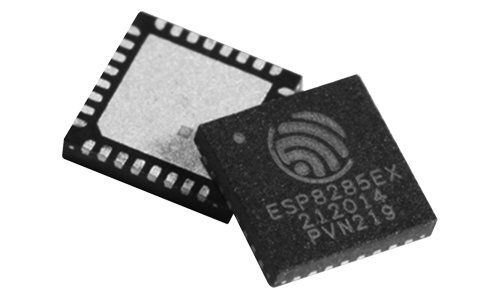
\includegraphics[width=150mm, keepaspectratio]{figures/esp8285.png}
	\caption{ESP8285 chip} 
\end{figure}

\begin{figure}[!ht]
	\centering
	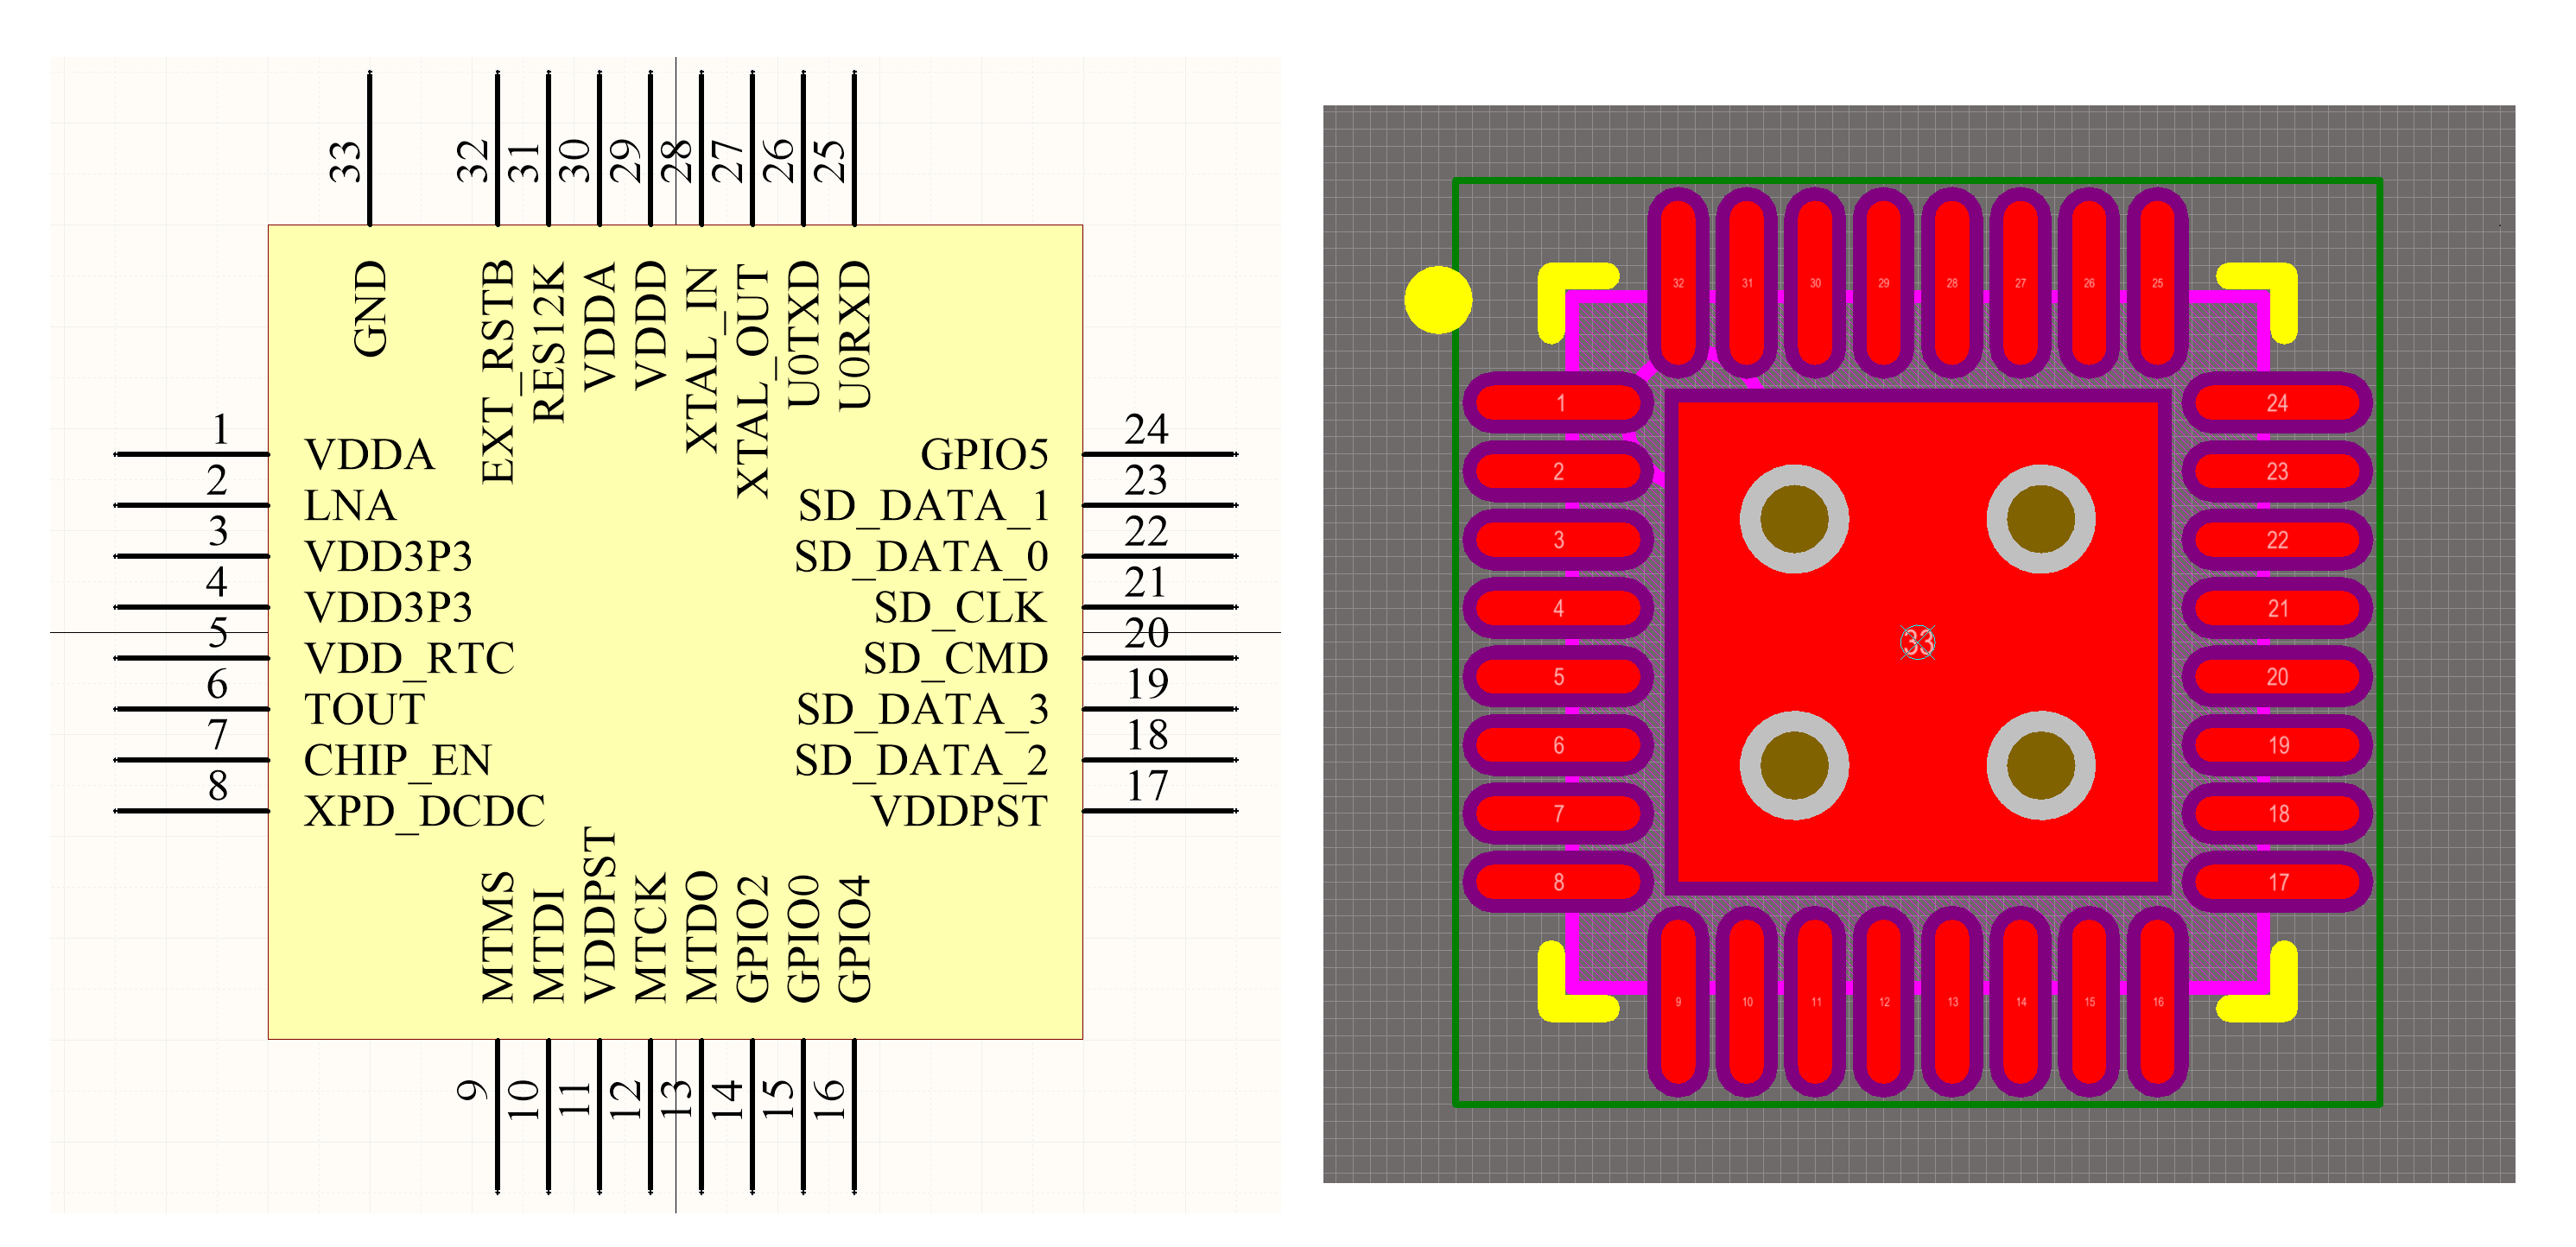
\includegraphics[width=150mm, keepaspectratio]{figures/esp8285-cad.png}
	\caption{ESP8285 chip CAD modellje}
\end{figure}

Az ESP8285 egy WiFi k�pes mikrokontroller teljes TCP/IP implement�ci�val, kifejezetten IOT (Internet of Things) alkalmz�sokhoz sz�nva. A chip 2016 nyar�n ker�lt forgalomba, de egy kor�bbi v�ltozat, az ESP8266 m�r 2014-�ta jelen van. Az egyetlen k�l�nbs�g az ESP8285-be integr�lt 1MB flash mem�ria, ami az esetek t�bbs�g�ben feleslegess� tette az ESP8266-n�l m�g sz�ks�ges k�ls� mem�riamodult. Emiatt mindk�t v�ltozat adatlapjai �s a le�r�sok is relev�nsak.
A chipcsal�d az ut�bbi id�ben nagy n�pszer\H{u}s�gre tett szert, k�sz�nhet�en annak, hogy a gy�rt� k�nai mellett angolul is el�rhet�v� tette a dokument�ci�t, illetve megnyitotta az SDK-t. 

Az ESP8285 modul kis m�ret\H{u}, �ra rendk�v�l kedvez� (2\$ k�r�l nagy t�telben), �s csak minim�lis kieg�sz�t� �ramk�rt ig�nyel, �s antennav�laszt�sn�l is nagy szabads�got enged a felhaszn�l�nak.

A modul magj�t egy Tensilica LX106 egys�g k�pzi, ami egy 80Mhz-en (opcion�lisan 160Mhz ig n�velhet�) 32 bites RISC architekt�rt�j� mikrokontroller. A chip alap�rtelmezettk�nt AT parancsokkal ir�ny�that�, soros portr�l vagy ak�r egy m�sik mikrokontrollerr�l. Komplexebb funkcionalit�s implement�l�s�ra is sz�mtalan lehet�s�g van. A legfontosabbak:

\begin{itemize}  
	\item GCC alap� toolchain (egy hivatalos gy�rt� �ltal fenntartott �s egy alternat�v v�ltozat)
	\item NodeMCU (IOT platform, Lua szkriptnyelven programozhat�)
	\item Arduino C++ platform 
	\item MicroPython (Python szkriptnyelv �rtelmez�)
\end{itemize}

Az egys�g a tervez�s szempontj�b�l legfontosabb tulajdons�gai, t�mogatott protokollok �s technol�gi�k: 

\begin{itemize} 
	\item 802.11 b/g/n/e/i t�mogat�s
	\item Wifi Direct (P2P)
	\item Titkos�t�si szabv�nyok hardveres gyors�t�sa
	\item+20 dBm ad�s
	\item-91 dbm v�tel
	\item Perif�ri�k: UART, SDIO, SPI, I2C, I2S, IR Remote Control, GPIO, ADC, PWM
	\item M\H{u}k�d�si fesz�lts�g: 3.0 V - 3.6 V
	\item Tokoz�s: QFN32-pin (5 mm x 5 mm)
	\item H�l�zati protokollok: IPv4, TCP, UDP, HTTP, FTP	
\end{itemize}

A Wifi-s kommunik�ci� egyik gyenge pontja az energiafogyaszt�s. A jelsug�rz�s nagy �ramfelv�tellel j�r egy�tt, illetve az �tlagfogyaszt�s is viszonylag magas. Ezen h�tr�ny kik�sz�b�l�s�re, ha az alkalmaz�si m�d lehet�v� teszi, a chip t�mogat t�bb energiak�m�l� m\H{u}k�d�si m�dot. A jellemz� fogyaszt�si adatok:

\begin{table}[ht]
	\footnotesize
	\centering
	\caption{ESP8285 fogyaszt�si adatai}
	\begin{tabular}{l r}
		M�d & Fogyaszt�s \\
		\hline
		Tx 802.11n (ad�s) & 170 mA\\

		Rx 802.11n (v�tel) & 56 mA\\

		Modem-Sleep & 15 mA\\
		
		Light-Sleep & 0.9 mA\\
		
		Deep-Sleep & 10 $\mu A$\\
		
		Kikapcsolva & 0.5 $\mu A$\\
	\end{tabular} 
\end{table}

%----------------------------------------------------------------------------
\subsection{Antenna}
%----------------------------------------------------------------------------

\begin{figure}[!ht]
	\centering
	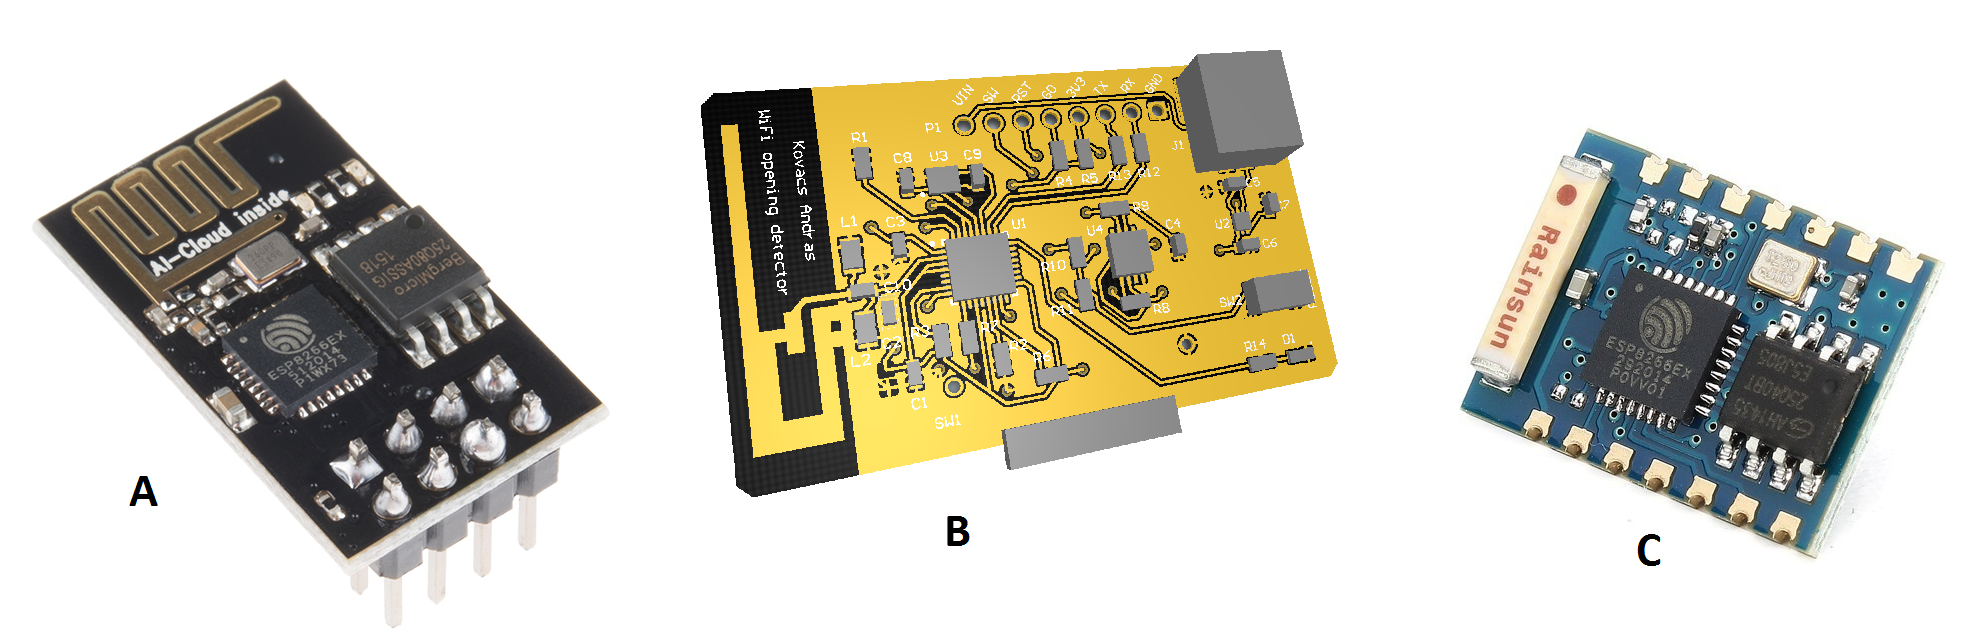
\includegraphics[width=150mm, keepaspectratio]{figures/antennas.png}
	\caption{Antenna megold�sok: Meander (A), Invert�lt F (B), Chip (C)}
\end{figure}

\begin{figure}[!ht]
	\centering
	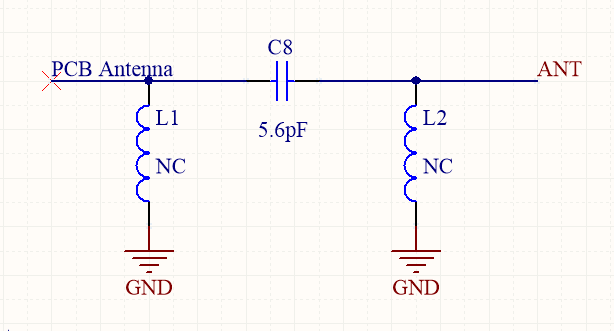
\includegraphics[width=150mm, keepaspectratio]{figures/antenna.png}
	\caption{Az illesztett antenna}
\end{figure}

A modulnak sz�ks�ge van k�ls� antenn�ra a WiFi kommunik�ci�hoz (2.4GHz). A legegyszer\H{u}bb �s legolcs�bb megold�s a nyomtatott �ramk�r�n elhelyezett antenna. Az antenn�t 50 $\Omega$ impedanci�hoz kell illeszteni. A leggyakoribb kialak�t�sok a \textbf{meander antenna} �s az \textbf{inverted-F antenna}.
Az el�bbi helyig�nye hozz�vet�legesen 1.5 cm az ut�bbi� 3 cm. Az ad�s min�s�ge jobb az inverted-F kialak�t�ssal, �s mivel a hely nekem rendelkez�sre �llt, e mellett d�nt�ttem. �gy illeszt�sre nem volt sz�ks�g, de mivel nyitva akartam hagyni m�s antenn�k kipr�b�l�s�nak a lehet�s�g�t is, ez�rt az �ramk�r�n elhelyezhet� k�t illeszt� induktivit�s.

Az antenna eszk�z karakterisztik�j�val kapcsolatban prec�z m�r�seket nem v�geztem, de a WiFi kapcsolat ak�r 20-30 m�ter t�vols�gb�l �s falon kereszt�l is stabil maradt.

%----------------------------------------------------------------------------
\subsection{K�telez� kieg�sz�t� elemek}
%----------------------------------------------------------------------------

Az IC el��ll�t mag�nak egy referencia�ramot, amihez sz�ks�ge van egy nagy pontoss�g� 12k$\Omega$-os ellen�ll�sra. A t�pfesz�lts�g sz\H{u}r�s�re egy 100nF-os, 1$\mu$F-os �s 10$\mu$F-os ker�miakondenz�tor h�rmast haszn�lok, az aj�nl�snak megfelel�en.

Az mikrokontroller k�ls� rezon�tor megl�t�t ig�nyli. A t�mogatott frekvenci�k 24MHz-t�l 40Mhz-ig terjednek. Mivel a WiFi-s kommunik�ci�n�l nem lehet jelent�s frekvenciahiba, v�lhet�en a rezon�tor pontatlans�g�ra alacsony a tolerancia. A nyomtatott �ramk�r�n �rdemes a rezon�torkrist�lyt min�l k�zelebb helyezni a mikrokontrollerhez, vi�k haszn�lata ellenjavallott. Mindh�rom eszk�zn�l egy Epson FA-128 26MHz-s krist�lyt haszn�ltam.

\begin{figure}[!ht]
	\centering
	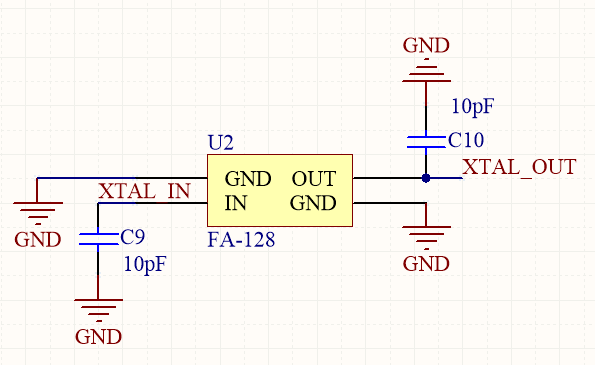
\includegraphics[width=150mm, keepaspectratio]{figures/resonator.png}
	\caption{A rezon�tor�ramk�r}
\end{figure}

%----------------------------------------------------------------------------
\section{T�pell�t�s}
%----------------------------------------------------------------------------

A tervez�si feladat r�sze volt minden egyes eszk�zh�z az optim�lis t�pell�t�si m�dot kiv�lasztani. A k�zponti egys�g �s a programozhat�
fali aljzat h�l�zati �ramr�l m\H{u}k�dik, m�g a k�rnyezeti szenzor �s a nyit�s�rz�kel� hordozhat� energiaell�t�st ig�nyel.

H�l�zatr�l t�pl�lva az extr�m takar�koss�g �rtelm�t vesz�ti. K�zenfekv� megold�snak t\H{u}nik egy egyben megvehet� kapcsol��zem\H{u} t�pegys�g alkalmaz�sa. A be�p�tett v�d�mechanizmusok �s a galvanikus lev�lasztotts�g el�ny. 

Az els� �s legk�zenfekv�bb megold�s a mobil eszk�z�kben rendk�v�l elterjedt Li-ion akkumul�tor. Energia �s teljes�tm�nys\H{u}r\H{u}s�gben is kiv�l�, nem m�rgez�, �s nem rendelkezik mem�riaeffektussal. T�lt�tts�g�t rendk�v�l lassan vesz�ti el. M�g kimer�lt �llapotban is k�pes 3V fesz�lts�get szolg�ltatni, ami azt jelenti, hogy 3-3.6V t\H{u}r�s\H{u} �ramk�r�kkel az akkumul�tor teljes kapacit�s�t ki tudom haszn�lni, �s elegend� egy cella. Mivel t�lt�s ut�n a cellafesz�lts�g el�rheti a 4.2V-ot, ez�rt az �ramk�r mindenk�pp v�delemre szorul. A Li-ion alap� megold�sok rendelkeznek h�tr�nyokkal is. T�lt�lt�s �s m�lykis�l�s ellen v�d��ramk�rt kell alkalmazni. Ennek hi�ny�ban a megold�s t\H{u}zvesz�lyes. Az akkumul�tor cella rendk�v�l s�r�l�keny, ez�rt sz�ks�g van a fizikai v�delemre. H�tr�nyk�nt eml�thet� m�g a Li-ion cella �reged�se is, de a legt�bb esetben, mire a teljes�tm�nycs�kken�s relev�ns� v�lik, maga a k�sz�l�g is elavul. Ha m�gis hossz� t�v� �zemre tervezn�nk, gondolni kell az akkumul�tor cser�lhet�s�g�re.

Alternat�va lehet h�rom darab 1.5V-os ceruzaelem haszn�lata is, de mivel ez esetben, ha nem akarok elfogadhatatlanul rossz hat�sfokot, valamilyen kapcsol��zem\H{u} t�pegys�get kell haszn�lnom, jelent�s m�ret\H{u} kieg�sz�t� �ramk�rrel. R�di�frekvenci�s alkalmaz�sokn�l jelent�s�ge van a t�pell�t�s zajmentess�g�nek is. Mivel a h�rom elem m�rete meghaladja azt a �ramk�r m�retet amit alkalmazni szeretn�k, ez�rt ezt a megold�st elvetend�nek gondolom.

Kis m�rete miatt felmer�het egy nem �jrat�lthet� Li-ion gombelem alkalmaz�sa is, els�dlegesen akkor, amikor fontos a kis m�ret �s s�ly, valamint a k�sz�l�k csak ritk�n, r�vid id�tartamokra van bekapcsolva. Mivel a WiFi ad� �ramfelv�tele r�videbb id�szakokban meghaladja a gombelem �ltal biztos�tott maximumot, ez�rt sz�ks�g van egy tov�bbi kondenz�tor elhelyez�s�re is, ami viszont nagyban semleges�ti ezen megold�s eredeti el�nyeit.

%----------------------------------------------------------------------------
\section{Az mikrokontroller felprogramoz�sa}
%----------------------------------------------------------------------------

Az mikrokontroller UART (Universal Asynchronous Receiver/Transmitter) protokollon kereszt�l programozhat�. A programoz�s �s bootol�s �zemm�d k�z�tti v�laszt�s a GPIO0 f�ldre illetve t�pra h�z�s�val �rhet� el. Alapvet�en k�t �letk�pes megold�st tudtam elk�pzelni:

\begin{itemize} 
	\item Az eszk�z�m integr�lva tartalmazza az USB/UART �talak�t�t, �s a GPIO0 �rt�k�t egy jumperrel lehet �ll�tani. A sz�m�t�g�pre csatlakoz�s egy micro USB porton kereszt�l oldom meg. Az USB/UART konverzi� feladat�ra n�pszer\H{u} megold�s az FTDI FT230X chip, legf�k�ppen apr� m�rete �s alacsony �ra miatt. 
	\item A sz�ks�ges l�bakat (GND, 3.3V, RX, TX, GPIO0) egy t�skessorra kivezetem, majd minim�lis kieg�sz�t� �ramk�rrel �s egy FTDI UMFT234XD USB portra kapcsolhat� fejleszt�k�rty�val programozom az eszk�zt.
\end{itemize}

Mindh�rom eszk�z eset�n az ut�bbi megold�st alkalmaztam. A program felt�lt�s�nek protokolj�ba m�lyebben nem tekintettem bele, mivel rendelkez�sre �lltak k�sz megold�sok (p�ld�ul az esptool.py szkript).

Nem kev�s probl�m�t okozott, hogy az alap�rtelmezett UART baud rate att�l f�gg hogy milyen frekvenci�j� rezon�tor ker�l felhaszn�l�sra. A felhaszn�l�i programban term�szetesen �ll�that� a frekvencia, de a bootol�skor kiadott st�tuszjel, �s felprogramoz�s sebess�ge is fix. Az a fix frekvencia oszcilloszk�ppal megm�rve 74880 Hz volt, ami nem egy szabv�nyos �rt�k (40 MHz-es oszcill�tor eset�n lenne 115200).

%----------------------------------------------------------------------------
\section{A nyomtatott �ramk�r�k}
%----------------------------------------------------------------------------

%----------------------------------------------------------------------------
\subsection{Alkatr�szek kiv�laszt�sa}
%----------------------------------------------------------------------------

Az alkatr�szek kiv�laszt�s�n�l els�dleges szempont volt, hogy a lehet� legkorszer\H{u}bb technik�val dolgozzak. Az ellen�ll�sokn�l, kondenz�torokn�l a 0603-as m�retet prefer�ltam, mivel az m�g k�zzel forraszthat�, de egy�ttal nagy s\H{u}r\H{u}s�gben helyezhet� el az �ramk�r�n. A rendel�sn�l az els�dleges forr�som a Mouser web�ruzh�z volt. A hatalmas v�lszt�k mellett az alkatr�szek tulajdons�gok szerint is j�l kereshet�ek voltak. A tervez�s sor�n tanulm�nyoztam hasonl� eszk�z�ket, illetve hobbist�knak sz�l� le�r�sokat is. Azon term�kek amelyekr�l ilyen m�don t�bbletinform�ci� �llt a rendelkez�semre, term�szetesen el�nyt �lveztek. Az adatlapokban megadott kieg�sz�t� �ramk�rre vonatkoz� aj�nl�sokat minden esetben betartottam. 

%----------------------------------------------------------------------------
\subsection{Tervez�s}
%----------------------------------------------------------------------------

A kapcsol�si rajzot, �s a nyomtattott �ramk�r terveket egyar�nt az Altium Designer tervez�szoftverrel k�sz�tettem el. Az alkalmaz�s az egyik legelterjedtebb, �s legt�bb funkci�val rendelkez� csomag a piacon, ez�rt a szerzett tapasztalatok k�s�bb rendk�v�l hasznosak lehetnek. A szoftver tanulm�nyi c�lokra ingyenesen el�rhet� volt. A ny�ktervez�s menete:

\begin{enumerate}  
	\item \textbf{A kapcsol�si rajz (Schematic) elk�sz�t�se:} Az alkatr�szeket szimb�lumok reprezent�lj�k. Ezen a tervez�si szinten az �sszek�ttet�sek l�trehoz�sa t�rt�nik meg. 
	\item \textbf{Szimul�ci� (opcion�lis):} Ha a komponensekhez k�sz�ltek m\H{u}k�d�si modellek, akkor az elk�sz�lt kapcsol�s viselked�se szimul�lhat�. 
	\item \textbf{A nyomtatott �ramk�r elk�sz�t�se:} Itt t�rt�nik a board alakj�nak defini�l�sa, az alkatr�szek �s huzaloz�s elhelyez�se. A helyess�g ellen�rz�se tervez�si szab�lyok (Design Rules) seg�ts�g�vel t�rt�nik.
	\item \textbf{A gy�rt�shoz sz�ks�ges file-ok el��ll�t�sa:} Ezut�n export�l�sra ker�lnek a gy�rt�shoz sz�ks�ges le�r�fileok. A Gerber file-ok tartalmazz�k az egyes r�tegekre (huzaloz�s, forraszt�sg�tl�s) vonatkoz� inform�ci�kat. A drill file defini�lja a furatok bev�g�sok hely�t.
\end{enumerate}

%----------------------------------------------------------------------------
\subsection{Gy�rt�s}
%----------------------------------------------------------------------------

Az elk�sz�lt ny�klaptervek az Elektronikai Technol�giai Tansz�k laborj�ban ker�ltek legy�rt�sra. K�t huzaloz�si r�tegn�l t�bbre nem volt sz�ks�g. Az el��rt 0.25mm-es szigetel�si k�zt p�r helyen, kis m�rt�kben meg kellett szegnem. A vi�khoz 0.5mm-es furatrokat alkalmaztam. 

\begin{figure}[!ht]
	\centering
	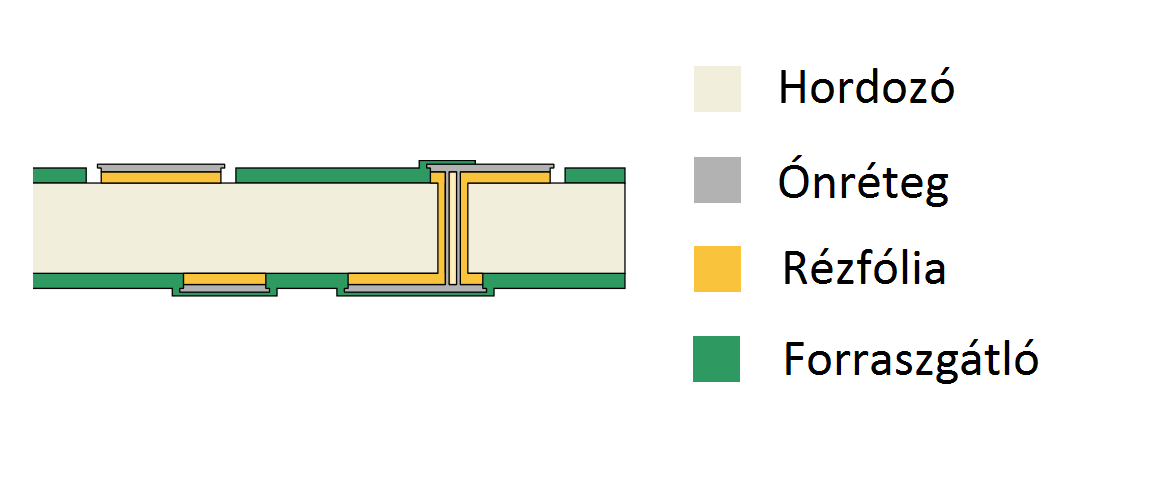
\includegraphics[width=150mm, keepaspectratio]{figures/pcb-layers.png}
	\caption{A nyomtatott �ramk�r fel�p�t�se} 
\end{figure}












%Status: under construction
%Todo: php Qt hozz�f�r�s
%----------------------------------------------------------------------------
\chapter{K�zponti egys�g}
%----------------------------------------------------------------------------

%----------------------------------------------------------------------------
\section{Hardver}
%----------------------------------------------------------------------------

Enn�l az egys�gn�l szerettem volna kipr�b�lni a Qt for Device Creation keretrendszert. A legjellemz�bb fel�p�t�s, hogy egy Linux rendszermagra �s egy ablakoz�rendszerre t�maszkodva fut a Qt-ban meg�rt szoftver. El�nye a teljes rugalmass�g, �s a gyors fejleszt�si �s tesztel�si ciklusok. H�tr�nya, hogy kicsivel er�sebb hardvert ig�nyel, mint az alacsony szinten meg�rt be�gyazott rendszerek, de a nagyobb teljes�tm�ny\H{u} SOC-ok (System on a Chip) olcs�v� v�l�sa ezt a faktort jelent�ktelenn� tette.

\begin{figure}[!ht]
	\centering
	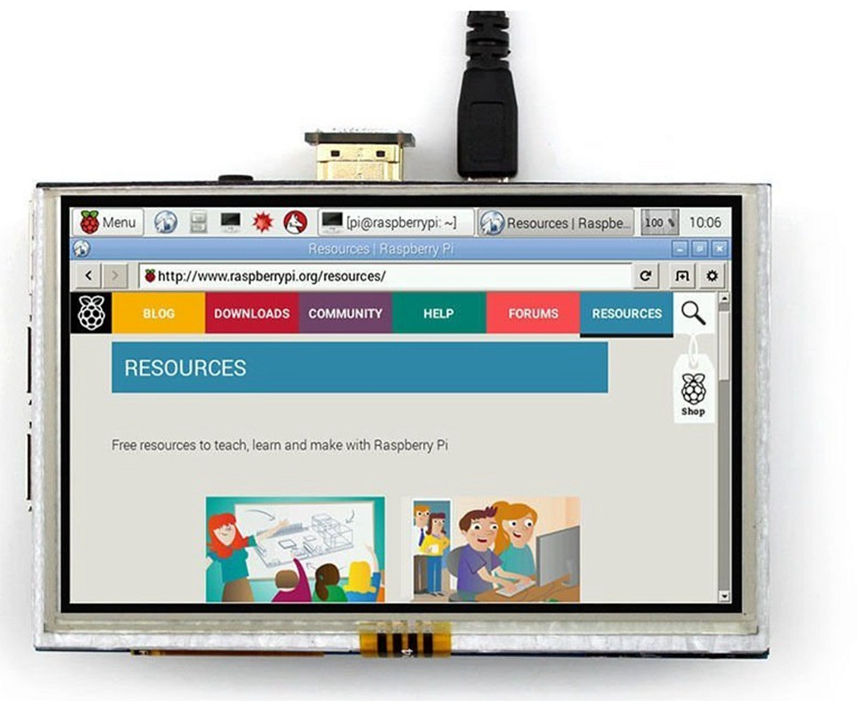
\includegraphics[width=150mm, keepaspectratio]{figures/rp3-and-display.png}
	\caption{Raspberry Pi 3 �rint�kijelz�vel } 
\end{figure}

%----------------------------------------------------------------------------
\subsection{Raspberry Pi 3}
%----------------------------------------------------------------------------

A Linux-ot futtat� board szerep�t egy Raspberry Pi 3 j�tsza. A feladathoz sz�ks�ges sz�m�t�si kapacit�s t�bbsz�r�s�vel rendelkezik, de mivel az elk�sz�lend� szoftver platformf�ggetlen, ez�rt k�s�bb t�meggy�rt�s eset�n egyszer\H{u}en portolhat� olcs�bb hardverre is. El�nye a 3-as verzi�nak, hogy nem ig�nyel WiFi modult, mivel m�r intergr�lva tartalmazza azt.

%----------------------------------------------------------------------------
\subsection{�rint�kijelz� (Elecrow 5 inch display for Raspberry Pi)}
%----------------------------------------------------------------------------

Olyan kijelz�t kerestem, aminek a m�rete m�r megfelel� egy ujjal kezelhet� interface kialak�t�s�hoz. A kijelz� legfontosabb tulajdons�gai:

\begin{itemize}  
	\item 800x480 TFT kijelz�
	\item HDMI k�pinterface
	\item Reziszt�v �rint�s�rz�kenys�g (SPI interface)
\end{itemize}

A beszerzett kijelz� meglehet�sen gyenge min�s�g\H{u}nek bizonyult. A �rint�si pontokat pontatlanul adta viszza, amint m�g kalibr�ci�val sem nagyon tudtam jav�tani. K�perny� betekint�si sz�gei gyeng�k, a sz�nek mosottak �s kontraszttalanok m�g szemb�l n�zve is. 


%----------------------------------------------------------------------------
\section{Szoftver}
%----------------------------------------------------------------------------

Mivel a k�zponti egys�g egy teljes �rt�k\H{u}, Linuxot (Raspbian Jessie) futtat� sz�m�t�g�pre, ez�rt technol�gi�k sz�les palett�j�b�l v�logathattam. A grafikus fel�let Qt keretrendszer seg�ts�g�vel k�sz�lt el. A tov�bbi webszerver funci�k megval�s�t�s�hoz a LAMP (Linux + Apache + MySQL + PHP) nagy n�pszer\H{u}s�gnek �rvend� megold�scsomagot haszn�ltam. Az egyszer\H{u}s�gn�l �s a kompakts�gn�l fontosabb szempont volt min�l t�bb ter�letr�l fejleszt�si tapasztalatot szerezni. 

%----------------------------------------------------------------------------
\subsection{Az alkalmaz�s}
%----------------------------------------------------------------------------


\begin{figure}[!ht]
	\centering
	
\includegraphics[width=150mm, keepaspectratio]{figures/placeholder.png}
	\caption{Az alkalmaz�s f�oldala} 
\end{figure}


\begin{figure}[!ht]
	\centering
	
\includegraphics[width=150mm, keepaspectratio]{figures/placeholder.png}
	\caption{Az alkalmaz�s (r�szleges) UML oszt�lydiagrammja} 
\end{figure}

%----------------------------------------------------------------------------
\subsubsection{Automatiz�l�s}
%----------------------------------------------------------------------------

Ki lehetne t\H{u}zni c�lul, hogy az rendelkez�sre �ll� eszk�z�ket felhszn�lva, b�rmilyen k�ztes logika leprogramozhat� legyen. M�sk�pp megfogalmazva, b�rmely besz�lt nyelven megfogalmazhat� egzakt m\H{u}k�d�s implement�lhat� legyen. Az inform�ci�elm�letben haszn�lt Turing teljess�g hasonl� tartalmat defini�l prec�zen.
Egy ilyen rendszer implement�l�sa meglehet?sen sok id�t vesz ig�nybe. Megold�s lehet valamely ECMAScript (Javascript) implement�ci� felhaszn�l�sa.
Qt keretrendszer alatt rendelkez�sre �ll QtScript modul (b�r elavultt� lett nyilv�n�tva), vagy b�rmely m�s modern motor, mint a Google V8-a vagy a Mozilla
SpiderMonkey-ja. Az eszk�z�k ekkor mint objektumok el�rhat�v� tehet?k.
Enn�l �n egy egyszer?bb, r�gz�tett sz�m� param�terb?l �ll� utas�t�sle�r� nyelvet val�s�tottam meg, a k�vetkez� adatokkal
\begin{itemize}  
	\item forr�s eszk�z azonos�t�ja
	\item forr�s param�ter (r�szletesen a \ref{sec:parameters} pontban)
	\item oper�tor: a forr�s param�ter �s a konstans k�z�tti logikai "<" �s ">" m?velet
	\item konstans: tetsz�leges sz�m
	\item utas�t�s
	\begin{itemize}
		\item link: a felt�tel logikai �rt�ke mindenkor megegyezik a c�lparam�terrel
		\item set: ha igazz� v�lik a felt�tel 1-re �ll�tja a c�lparam�tert
		\item reset: ha hamiss� v�lik a felt�tel 0-re �ll�tja a c�lparam�tert
	\end{itemize}
	\item c�l eszk�z azonos�t�ja
	\item c�l param�ter	(r�szletesen a \ref{sec:parameters} pontban)
\end{itemize}






%----------------------------------------------------------------------------
\subsection{A webszerver}
%----------------------------------------------------------------------------

Az IOT egyik alapelve a megl�v� webes szabv�nyok alkalmaz�sa, ez�rt a k�zponti egys�g egy teljes �rt�k\H{u} webszervert val�s�t meg. Ehhez az Apache HTTP Server \cite{wiki-apache} ny�lt forr�sk�d� alkalmaz�st vettem ig�nybe, kieg�sz�tve a PHP \cite{wiki-php} (PHP: Hypertext preprocessor) modullal. Mivel az �sszes rendelkez�sre �ll� adat egy adatb�zisban t�rol�dik, ez�rt ak�r a grafikus alkalmaz�st�l teljesen f�ggetlen�l, b�rmely funkci� tiszt�n webes alapon is implement�lhat�.

A m\H{u}k�d�hez l�tfontoss�g� egyetlen funkci� a nyit�s�rz�kel� modul sz�m�ra ny�jtott interface, melyet a k�vetkez� PHP k�d val�s�t meg:

\lstinputlisting[language=PHP]{source/opendetectorPhp.txt}

%8398241 ambient < 10 set 8396086 relay
%8398241 temperature > 30 link 8398241 ledamber


%----------------------------------------------------------------------------
\subsection{Az adatb�zis}
%----------------------------------------------------------------------------

A grafikus alkalmaz�s, az alapvet� konfigur�ci�n k�v�l nem t�rol adatot, ehelyett azokhoz lek�rdez�seken kereszt�l jut hozz�. Ehhez a MySQL \cite{wiki-mysql} rel�ci�s adatb�ziskezel� rendszer�t haszn�lom. Az okosotthon rendszerhez egy k�l�n adatb�zist hoztam l�tre \textbf{smarhome} alap�rtelmezett n�vvel, a k�vetkez� t�bl�kkal:

\begin{table}[ht]
	\footnotesize
	\centering
	\caption{A nyit�s�rz�kel� adatb�zis strukt�r�ja: \textbf{opendetector}}
	\begin{tabular}{|l|l|l|l|}
		\hline
		\textbf{N�v} & \textbf{T�pus} & \textbf{Extra} & \textbf{Le�r�s} \\ 
		\hline
		ID & int & AUTO\_INCREMENT & a bejegyz�s azonos�t�ja \\
		\hline
		DEVICE & int &  & az eszk�z azonos�t�ja \\
		\hline
		OPEN & tinyint &  & 0:csukott 1:nyitott �llapot \\
		\hline
		TIMESTAMP & timestamp & CURRENT\_TIMESTAMP & a bejegyz�s d�tuma �s ideje \\
		\hline
	\end{tabular} 
\end{table}

\begin{table}[ht]
	\footnotesize
	\centering
	\caption{A k�rnyezeti szenzor adatb�zis strukt�r�ja: \textbf{envirnmentalsensor}}
	\begin{tabular}{|l|l|l|l|}
		\hline
		\textbf{N�v} 	& \textbf{T�pus} 	& \textbf{Extra} & \textbf{Le�r�s} \\ 
		\hline
		ID & int & AUTO\_INCREMENT & a bejegyz�s azonos�t�ja \\
		\hline
		DEVICE & int &  & az eszk�z azonos�t�ja \\
		\hline
		TIMESTAMP & timestamp & CURRENT\_TIMESTAMP & a bejegyz�s d�tuma �s ideje \\
		\hline
		TEMP & decimal &  & H�m�rs�klet \\
		\hline
		PRESS & decimal &  & L�gnyom�s \\
		\hline
		HUM & decimal &  & P�ratartalom \\
		\hline
		AMB & decimal &  & K�rnyezeti f�ny \\
		\hline
		R & int &  & piros csatorna sz�ml�l�ja \\
		\hline
		G & int &  & z�ld csatorna sz�ml�l�ja \\
		\hline
		B & int &  & k�k csatorna sz�ml�l�ja \\
		\hline
		W & int &  & feh�r csatorna sz�ml�l�ja \\
		\hline
	\end{tabular} 
\end{table}

\begin{table}[ht]
	\footnotesize
	\centering
	\caption{A programozhat� aljzat adatb�zis strukt�r�ja: \textbf{wifisocket}}
	\begin{tabular}{|c|c|c|c|}
		\hline
		\textbf{N�v} 	& \textbf{T�pus} 	& \textbf{Extra} & \textbf{Le�r�s} \\ 
		\hline
		ID & int & AUTO\_INCREMENT & a bejegyz�s azonos�t�ja \\
		\hline
		DEVICE & int &  & az eszk�z azonos�t�ja \\
		\hline
		TIMESTAMP & timestamp & CURRENT\_TIMESTAMP & a bejegyz�s d�tuma �s ideje \\
		\hline
		POWER & decimal &  & a felvett teljes�tm�ny \\
		\hline
		VOLTAGE & decimal &  & a m�rt fesz�lts�g \\
		\hline
		CURRENT & decimal &  & a m�rt �ram \\
		\hline
		POWERFACTOR & decimal &  & a teljes�tm�nyt�nyez� \\
		\hline
	\end{tabular} 
\end{table}

\begin{table}[ht]
	\footnotesize
	\centering
	\caption{A logol�shoz haszn�lt adatb�zis strukt�ra: \textbf{log}}
	\begin{tabular}{|c|c|c|c|}
		\hline
		\textbf{N�v} 	& \textbf{T�pus} 	& \textbf{Extra} & \textbf{Le�r�s} \\ 
		\hline
		ID & int & AUTO\_INCREMENT & a bejegyz�s azonos�t�ja \\
		\hline
		DEVICE & int &  & az eszk�z azonos�t�ja \\
		\hline
		TIMESTAMP & timestamp & CURRENT\_TIMESTAMP & a bejegyz�s d�tuma �s ideje \\
		\hline
		LOGLEVEL & tinyint &  & a log t�pusa \\
		\hline
		MESSAGE & text &  & a logolt �zenet \\
		\hline
	\end{tabular} 
\end{table}


Az \textbf{envirnmentalsensor} �s \textbf{wifisocket} t�bl�k egyszer\H{u}en az eszk�zr�l t�rt�nt egy leolvas�s eredm�ny�t t�rolj�k, megl�t�k nem l�tfontoss�g�, a legt�bb esetben elegend� a legfrissebb adat, ami tetsz�leges id?ben lek�rdezhet�. Ezzel szemben az nyit�s�rz�kel�k �llapota egyed�l a \textbf{opendetector} t�bl�b�l olvashat� ki, mivel az eszk�z csak �llapotv�ltoz�s (nyit�s, csuk�s) eset�n �bred fel, egy bejegyz�s megt�tel�nek erej�ig.

A \textbf{log} t�bl�t egyed�l debugol�s c�lj�ra haszn�ltam, de speci�lis LOGLEVEL byte �rt�kek lefoglal�s�val ak�r postal�da jelleg\H{u} kommunik�ci� is implement�laht� az eszk�z�k k�z�tt.

%----------------------------------------------------------------------------
\section{Alternat�v�k}
%----------------------------------------------------------------------------

C�l volt az, hogy az egyes eszk�z�k a lehet� legkev�sb� f�ggjenek a k�zponti egys�gt�l. Nyitva akartam hagyni annak a lehet�s�g�t is, hogy ezen r�szegys�g funkcionalit�sa impement�lhat� legyen b�rmilyen alternat�v eszk�zre mint p�ld�ul egy androidos okostelefon, egy iPad, vagy ak�r egy b�ng�sz�. Ennek �rdek�ben p�ld�ult a h�m�rs�klet JSON form�tumban is el�rhet�.




%Status: 8 lorems
%Todo: bevezet�, specifik�ci� sz�veges�t�se, hardware bevezet�, weblap (root)

%----------------------------------------------------------------------------
\chapter{Programozhat� aljzat �ramm�r�vel}
%----------------------------------------------------------------------------

%----------------------------------------------------------------------------
\section{Specifik�ci�}
%----------------------------------------------------------------------------

\begin{figure}[!ht]
	\centering
	\begin{minipage}{0.45\textwidth}
		\centering
		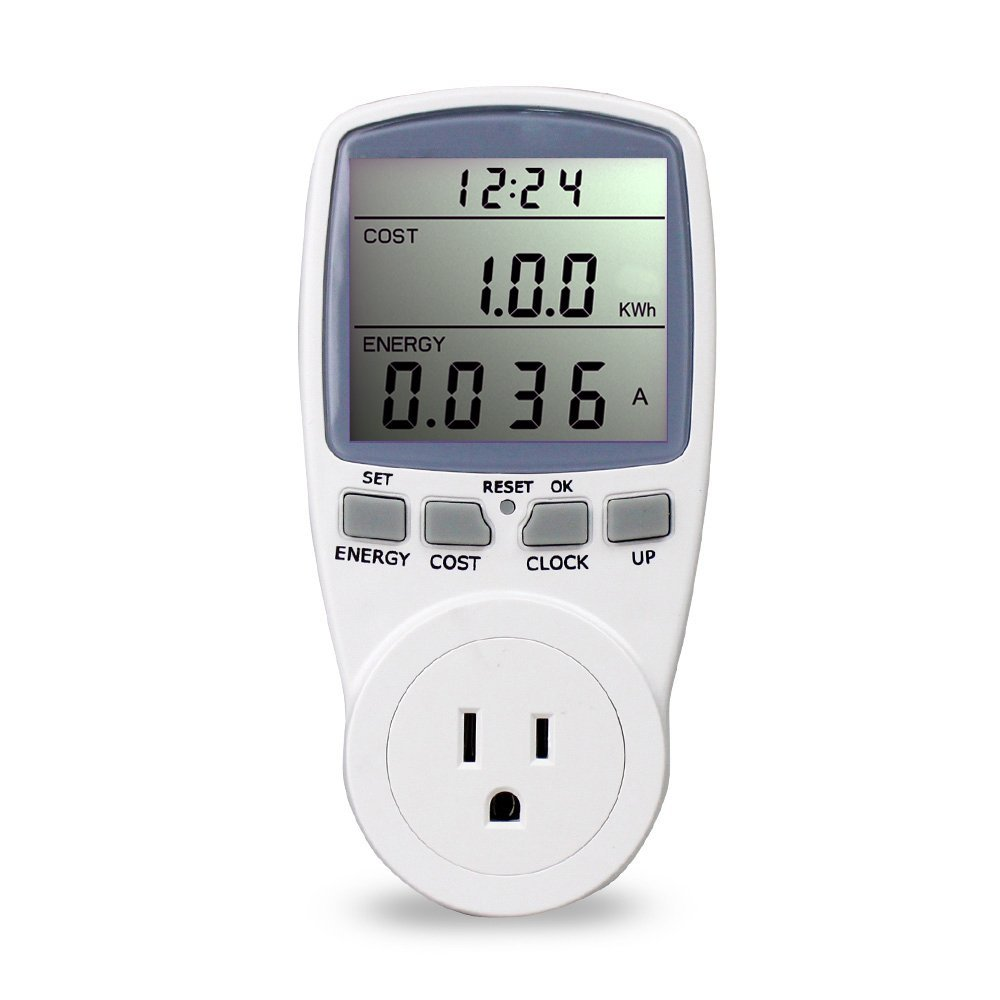
\includegraphics[width=0.9\textwidth]{figures/socket-energie-metering.jpg} % first figure itself
		\caption{Aljzat teljes�tm�nym�r�ssel}
		\label{fig:existing-socket-powermeter}
	\end{minipage}\hfill
	\begin{minipage}{0.45\textwidth}
		\centering
		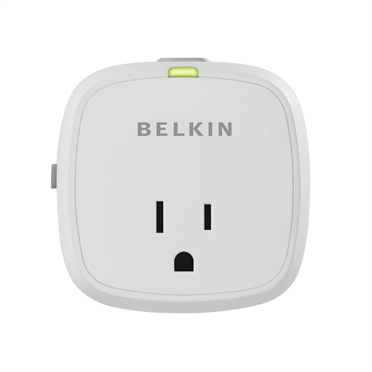
\includegraphics[width=0.9\textwidth]{figures/socket-w-wifi.png} % second figure itself
		\caption{WiFi-s konnektor}
		\label{fig:existing-socket-wifi}
	\end{minipage}
\end{figure}

\begin{figure}[!ht]
	\centering
	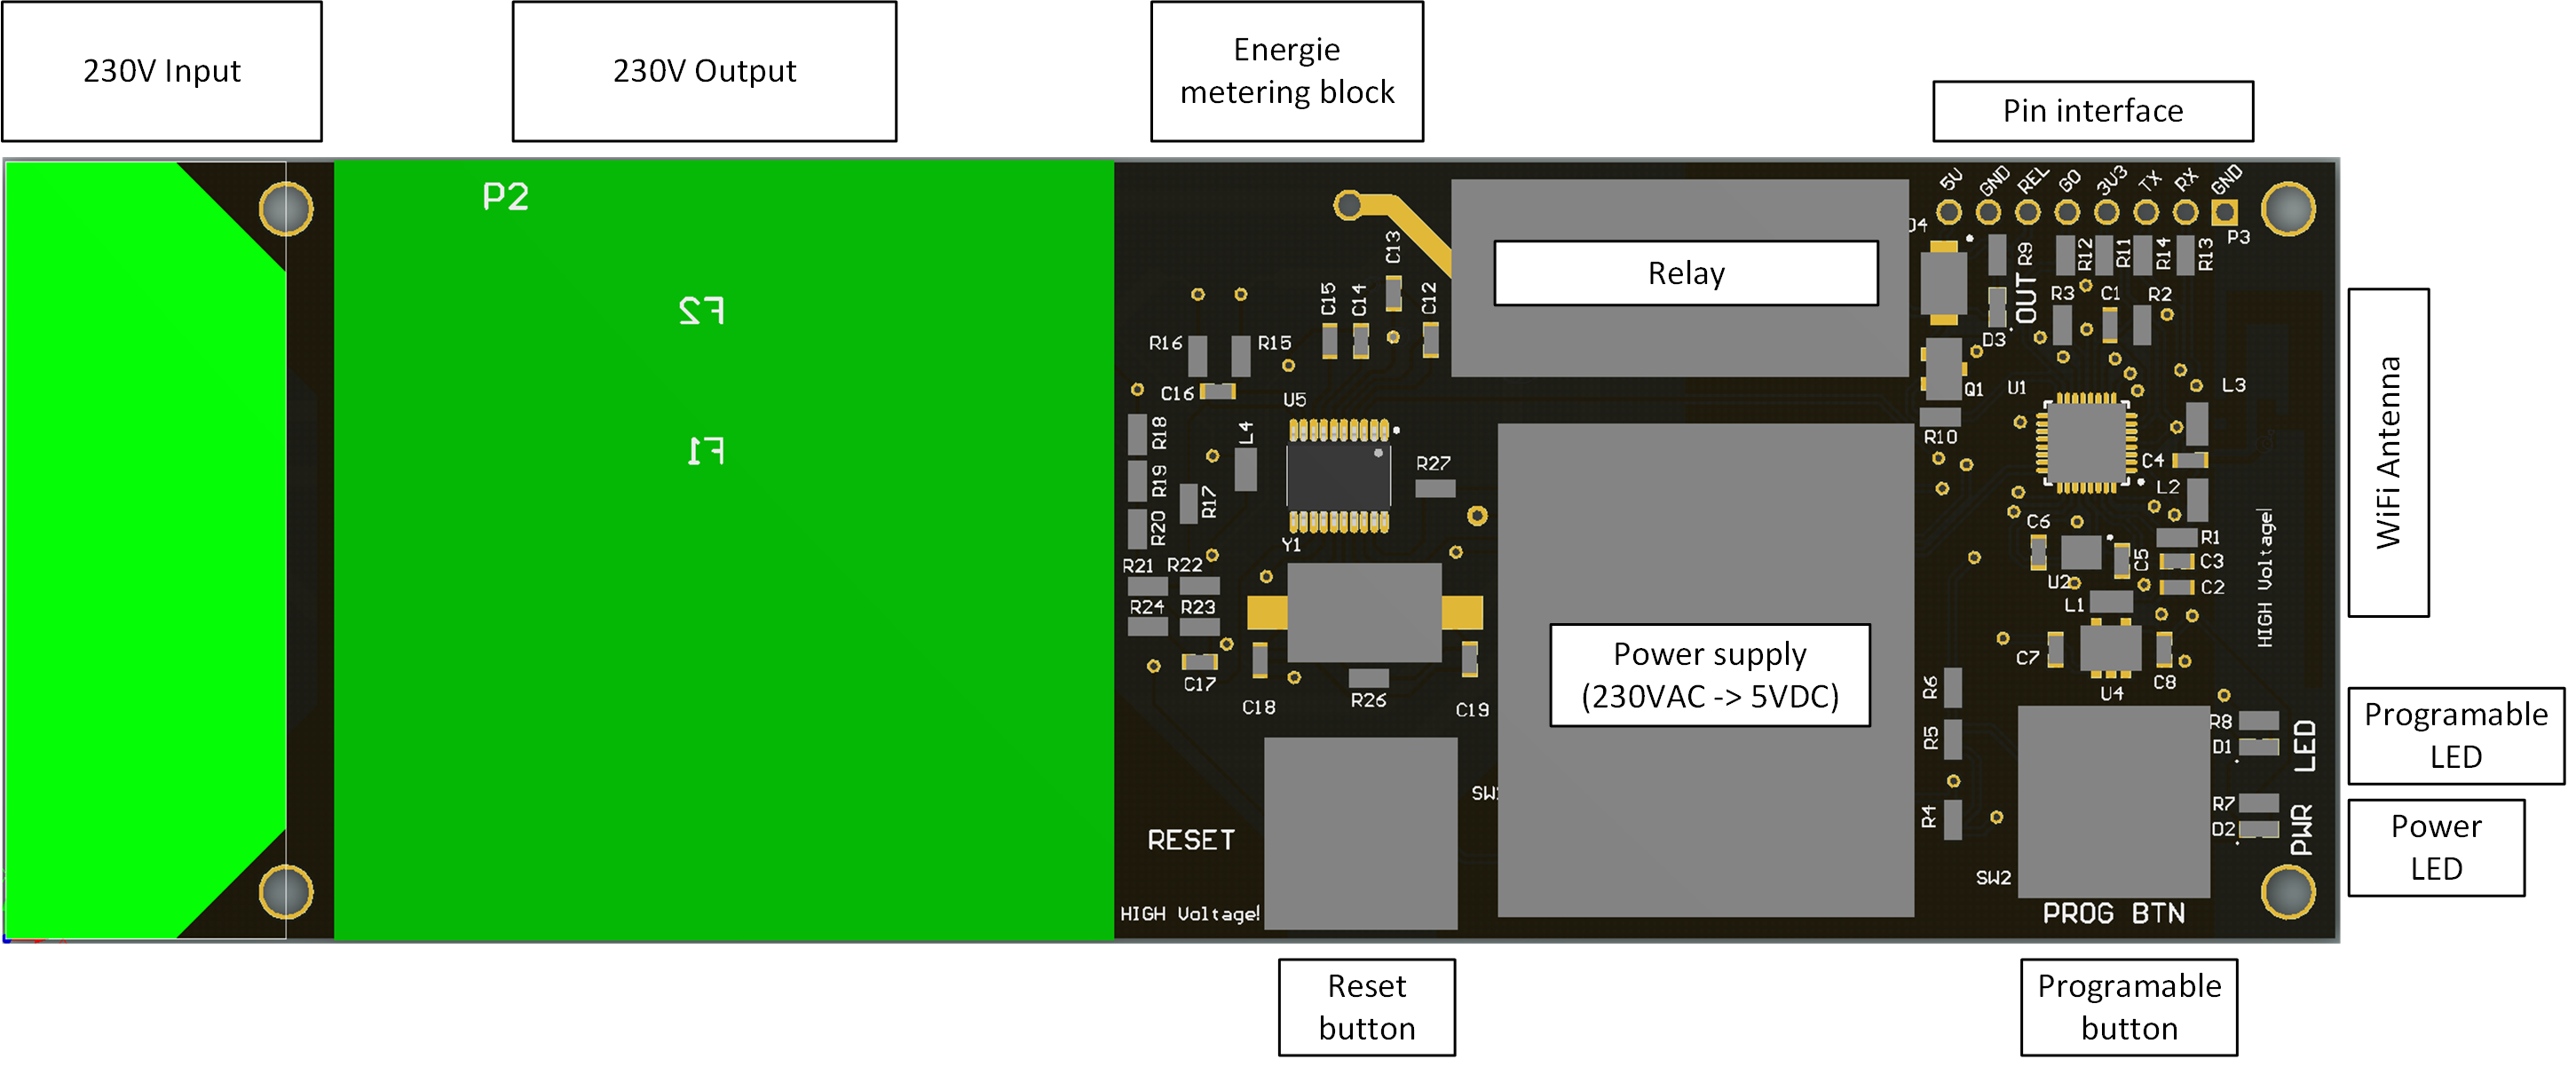
\includegraphics[width=150mm, keepaspectratio]{figures/wifisocket-blocks.png}
	\caption{A programozhat� aljzat blokkdiagramja}
	\label{fig:wifisocket-blockdiagram} 
\end{figure}




A piacon rengeteg kapcsolhat� �s teljes�tm�nym�r�s aljzat �s hosszab�t� tal�lhat� meg (\ref{fig:existing-socket-powermeter}, \ref{fig:existing-socket-wifi}-es �br�k). Lehets�ges, hogy l�tezik, de nekem nem siker�lt olyat tal�lnom ami:

\begin{itemize}  
	\item megfizethet� (30\$-40\$)
	\item k�pes a h�l�zati fesz�lts�get ki �s bekapcsolni, tetsz�leges logika alapj�n
	\item teljes�tm�nyt m�r nagy pontoss�ggal (bele�rtve a teljes�tm�nyt�nyez�t)
\end{itemize}

Egy programozhat� aljzat seg�ts�g�vel nem okos eszk�z�k is okoss� alak�that�ak (ki �s bekapcsolhat�s�g erej�ig). Az eszk�z�mn�l az egy kimenet\H{u} modul�ris hosszab�t� kialak�t�s mellett d�nt�ttem (\ref{fig:wifisocket-blockdiagram}-as �bra). 


%----------------------------------------------------------------------------
\section{Hardver}
%----------------------------------------------------------------------------

\begin{table}[ht]
	\footnotesize
	\centering
	\caption{A k�rnyezeti szenzor alkatr�sz list�ja}
	\begin{tabular}{|c|c|c|c|c|c|}
		\hline
		& \textbf{Db.} 	& \textbf{Le�r�s} 	& \textbf{Felh.} 	& \textbf{Gy�rt�} 	& \textbf{Azonos�t�} \\ 
		\hline
		1 & 1 & WiFi-s mikrokontroller & U1 & Espressif & ESP8285 \\
		\hline
		2 & 1 & Rezon�tor krist�ly & U2 & Epson & FA-128 26Mhz \\
		\hline		
		3 & 1 & Nyom�gomb & SW1 & CandK Components & D6C90 F2 LFS \\
		\hline
		4 & 3 & LED (0603) & D1..3 & Panasonic & LNJxxx \\
		\hline
		5 & 3 & Olvad�biztos�t�k & F1,F2 & Shurter & 3403.0173.11 \\
		\hline
		6 & 1 & Rel� & SW1 & TE Connectivity & RTE24005 \\
		\hline
		7 & 1 & Tranzisztor & Q1 & ON Semiconductor & MMBT2222ALT1G \\
		\hline
		8 & 1 & Egyenir�ny�t� & D4 & Rectron & FM4007W-W \\
		\hline
		9 & 1 & T�pegys�g 230AC->5V & x & Vigortronix & VTX-214-003-105 \\
		\hline
		10 & 1 & Buck 5V->3.3V & U4 & TI & LM3670MF-3.3 \\
		\hline
		11 & 1 & Header & P1 & Omron & XG8V-0831 \\ 
		\hline
		12 & 1 & Teljes�tm�ny m�r� IC & U3 & ST & STPM10BTR \\
		\hline
		13 & 1 & Rezon�tor krist�ly & Y1 & Abracon & ABLS-4.194304MHZ \\
		\hline
		14 & 1 & �ramm�r� s�nt & R25 & Wishay & WSLP5931 \\
		\hline
		15 & 1 & AC Csatlakoz� & P1 & Qualtek & 703W-00/54 \\
		\hline
		16 & 1 & AC Foglalat & P2 & x  & x \\
		\hline
		17 & 26 & Ellen�ll�s (0603) & R1..26 & Viking Tech Corp. & - \\
		\hline
		18 & 19 & Kondenz�tor (0603) & C1..19 & Yageo, Samsung & - \\
		\hline

	\end{tabular} 
\end{table}

%----------------------------------------------------------------------------
\subsection{T�pell�t�s}
%----------------------------------------------------------------------------

\begin{figure}[!ht]
	\centering
	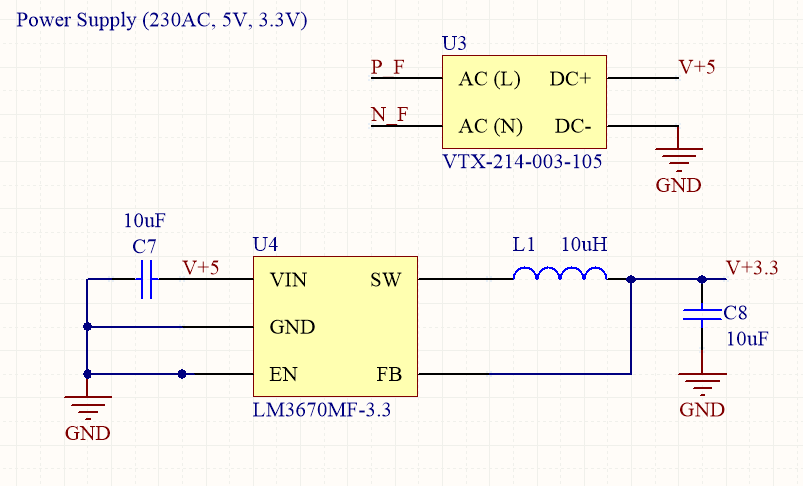
\includegraphics[width=150mm, keepaspectratio]{figures/wifisocket-power-supply.png}
	\caption{A t�p�ramk�r} 
\end{figure}

Ez az egys�g a m\H{u}k�d�s�hez sz�ks�ges energi�t 230V-os h�l�zatb�l veszi fel. A teljes�tm�nym�r� chip �s a WiFi-s mikrokontroller 3.3V is t�pell�t�st kap, mig a rel� meghajt�s�hoz 5V-ra van sz�ks�g.

%----------------------------------------------------------------------------
\subsubsection{Vigortronix VTX-214-003-105 \cite{vtx-214-003-105-ds}}
%----------------------------------------------------------------------------

\begin{figure}[!ht]
	\centering
	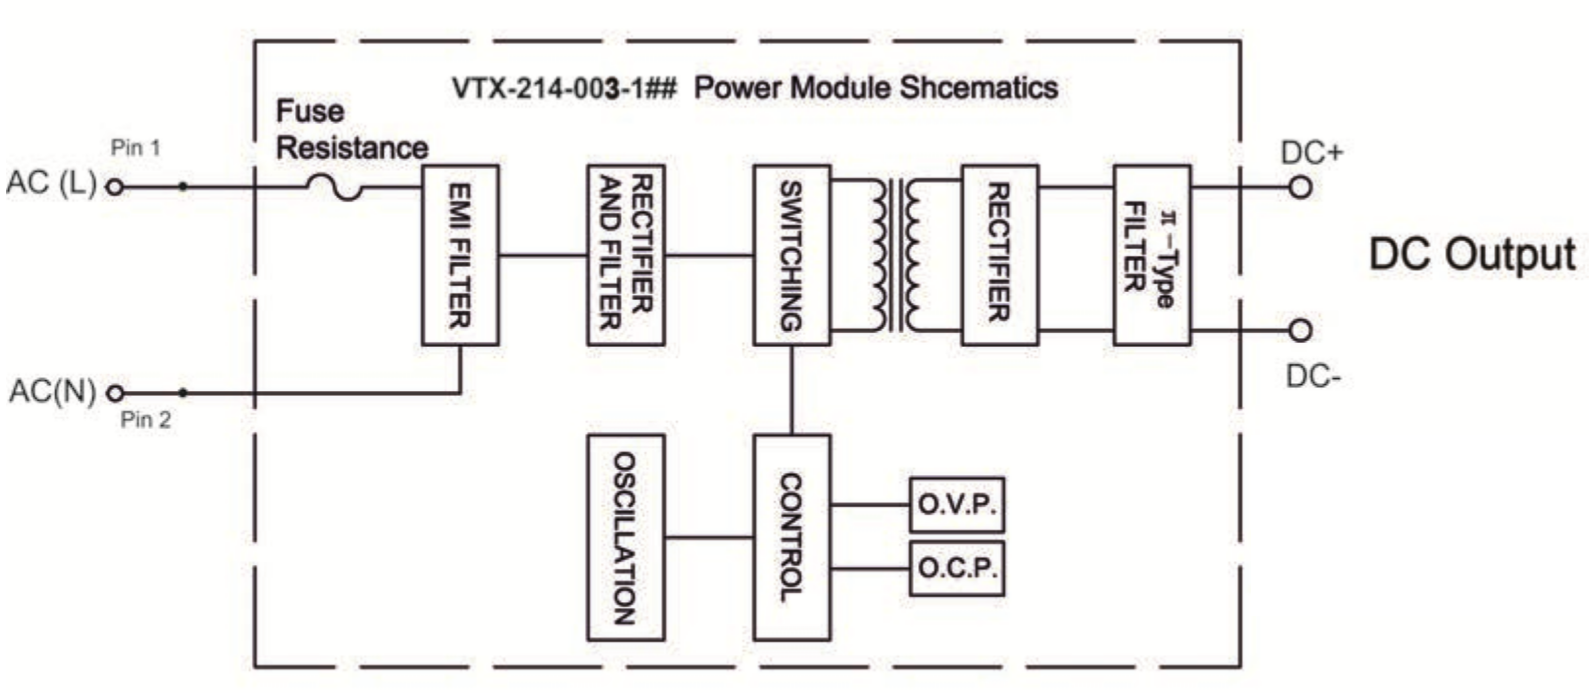
\includegraphics[width=150mm, keepaspectratio]{figures/vigortronix-block.png}
	\caption{Az VTX-214-003-105 blokkv�zlata}
	\label{fig:vtx-214-003-105-block}
\end{figure}

A Vigortronix VTX konvertersorozat�r�l sajnos korl�tozott r�szletess�g\H{u} dokument�ci� �ll rendelkez�sre. A t�pegys�g teljesen lev�lasztott, integr�lt, a \ref{fig:vtx-214-003-105-block}-es �br�n l�that�, hogy semmif�le kieg�sz�t� �ramk�rt nem ig�nyel. Topol�gi�j�t tekintve lev�lasztott kapcsol��zem\H{u} t�pegys�g. A legfontosabb jellemz�i:

\begin{itemize}  
	\item 5V egyenfesz�lts�g a kimeneten
	\item 600mA kimeneti �ram
	\item 100 VAC-t�l 275VAC-ig terjed� bemeneti fesz�lts�g
	\item 47Hz - 63Hz bemeneti frekvencia
	\item alacsony hull�moss�g �s zaj
	\item 4200Vrms - es izol�c�
	\item Hiccup mehanizmus (r�vid id�re le�ll) t�lterhel�s eset�n
	\item 70\% feletti hat�sfok
	\item 30g-os s�ly	
\end{itemize}




%----------------------------------------------------------------------------
\subsubsection{Texas Instruments LM3670MF-3.3 \cite{lm3670mf-ds}}
%----------------------------------------------------------------------------

\begin{figure}[!ht]
	\centering
	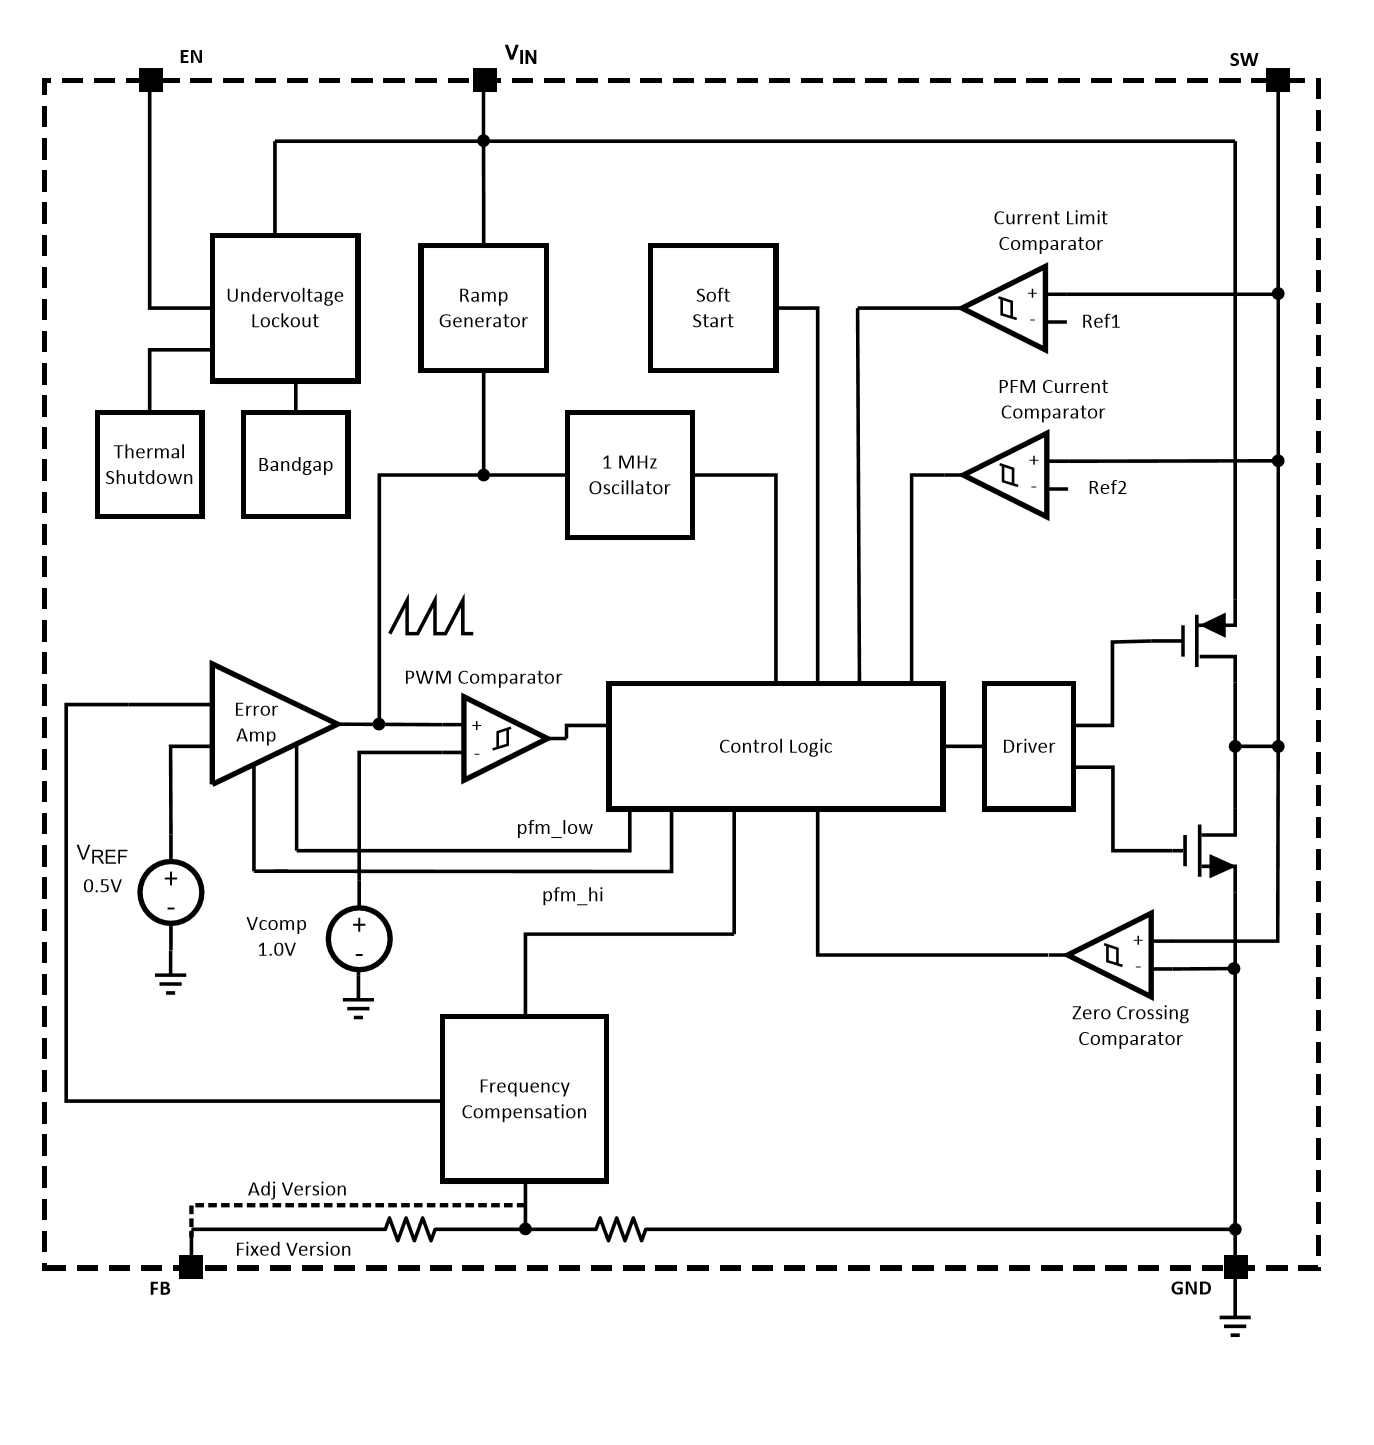
\includegraphics[width=150mm, keepaspectratio]{figures/lm3670-func-block.png}
	\caption{Az LM3670MF funkcion�lis blokkdiagramja}
\end{figure}

A Texas Instruments LM3670 sorozata egy DC-DC szinkron step-down (buck) konverter, els�sorban mobil eszk�z�kre optimaliz�lva. A kimenet�t (esetemben 3.3V) 5.5V �s 3.3V k�z�tt k�pes tartani (low dropout mode). A konverter extr�m magas, hozz�vet�legesen 95\%-os hat�sfokot ny�jt. Az tipikus terhel�s melletti 1MHz-es kapcsol�si frekvencia miatt elegend� h�rom (k�t kondez�tor �s egy induktivit�s) apr� fel�letszerelt elem a chip m\H{u}k�dtet�s�hez. Annak �rdek�ben, hogy alacsony �ram mellett se cs�kkenjen a hat�sfok, az vez�rl�s PWM-r�l (Pulse Width Modulation) PFM-re (Pulse Frequency Modulation) v�lt.

%----------------------------------------------------------------------------
\subsection{Teljes�tm�nym�r�s}
%----------------------------------------------------------------------------

\begin{figure}[!ht]
	\centering
	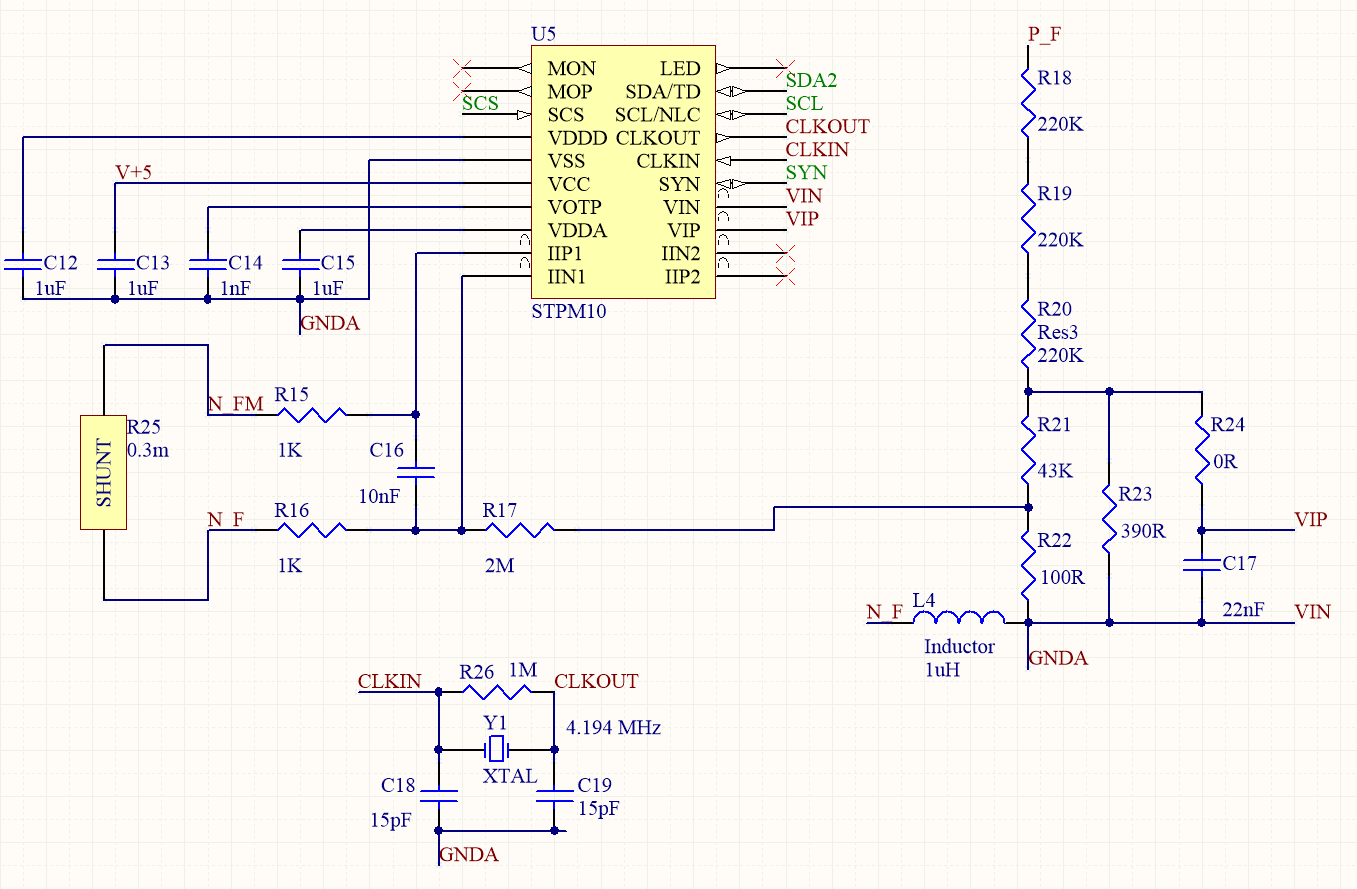
\includegraphics[width=150mm, keepaspectratio]{figures/wifisocket-power-meter.png}
	\caption{Az teljes�tm�nym�r�s�rt felel�s �ramk�rr�szlet} 
\end{figure}

A teljes�tm�nym�r�shez sz�ks�ges a fesz�lts�g �s az �ram folyamatos mintav�telez�se, mivel nem garant�lhat� a tiszta ohmos terhel�s. A jellemz�k m�r�s�re ak�r haszn�lhat� �ltal�nos c�l� mikrokontroller is, de val�sz�n�s�thet�, hogy komolyabb jelkondicion�l�s �s el�er�s�t�s n�lk�l a pontoss�g m�g az 1\%-ot sem �ri el. Mivel az �ltalam haszn�lt mikrokontroller am�gy sem volt alkalmas a feladatra, ez�rt az ST STPM10BTR IC-j�t vettem ig�nybe a teljes�tm�nym�r�shez.

%----------------------------------------------------------------------------
\subsubsection{ST STPM10BTR \cite{stpm10-ds}}
%----------------------------------------------------------------------------

\begin{figure}[!ht]
	\centering
	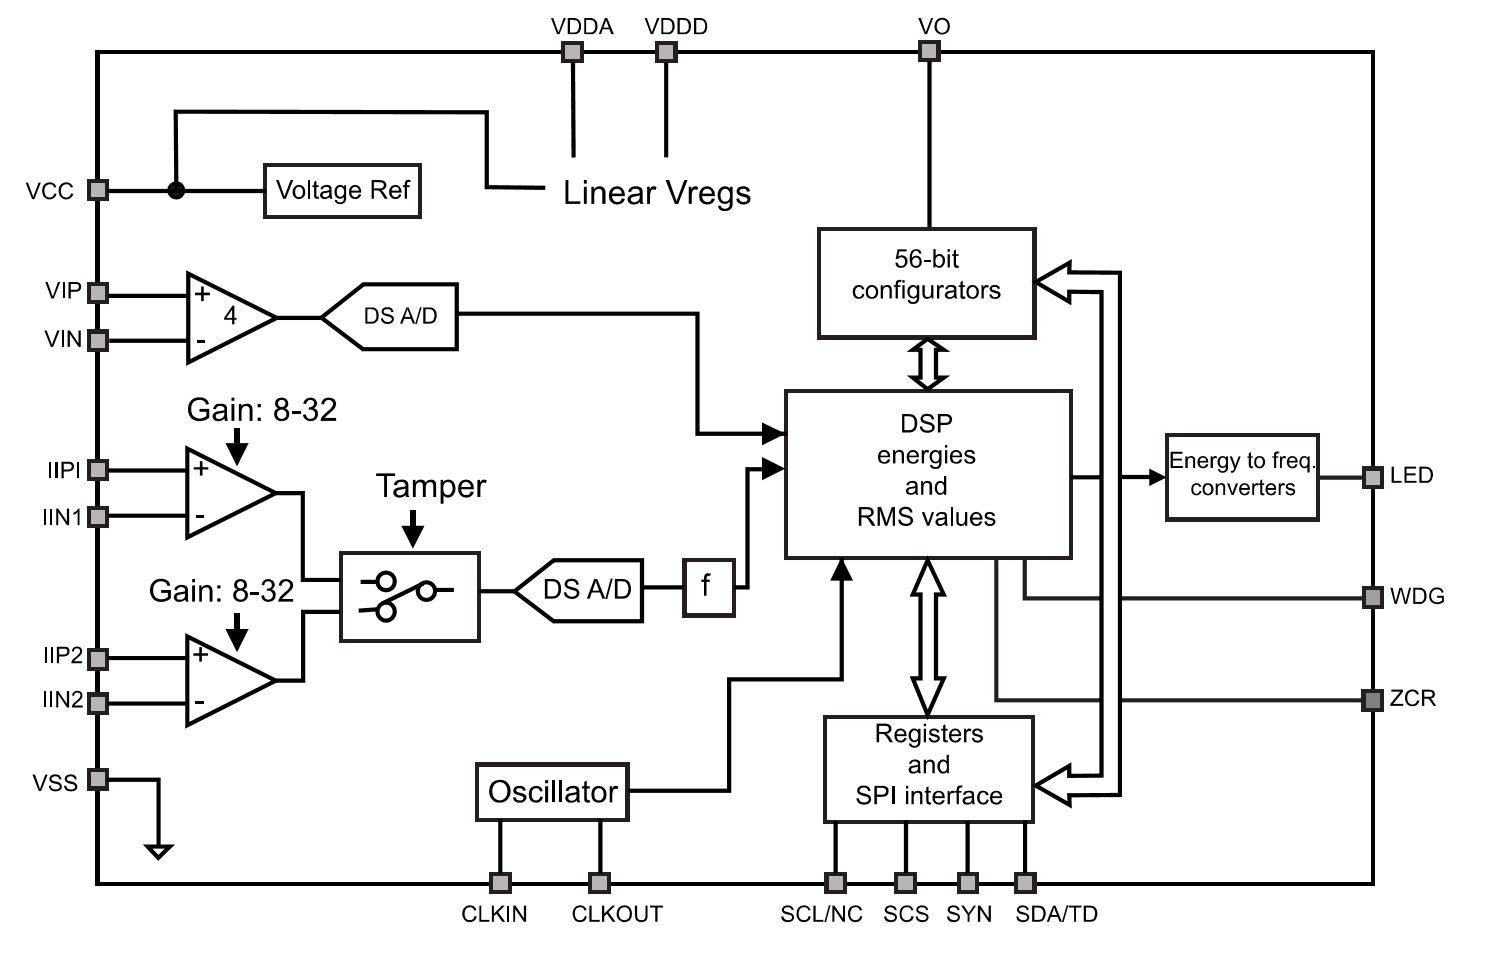
\includegraphics[width=150mm, keepaspectratio]{figures/stpm10-block.png}
	\caption{Az STPM10BTR blokkv�zlata} 
\end{figure}

Az ST STPM10BTR egy programozhat�, egyf�zis� teljes�tm�nym�r� IC. K�pes hat�sos, medd� �s l�tsz�lagos teljes�tm�ny m�r�s�re. Az hat�sos teljes�tm�nyt k�t r�szre osztja:

\begin{itemize}
	\item 0. t�pus: csak az alapharm�nikus �ltal felvett teljes�tm�ny
	\item 1. t�pus: a felharm�nikusok �ltal felvett teljes�tm�ny 
\end{itemize}

Az �ramnak �s a fesz�lts�gnek el�rhet� a pillanatnyi �s a n�gyzetes k�z�p�rt�ke, valamint m�r�sre ker�l a h�l�zati frekvencia is. 

A fesz�lts�gm�r�shez a h�l�zati fesz�lts�g sz\H{u}rt �s leosztott v�ltozat�t kell bevezetni az IC-be, figyelembe v�ve, hogy a bemenet 0.3V-ig toler�ns. A k�v�nt oszt�s el�r�s�hez prec�zi�s ellen�ll�sokat haszn�ltam. Term�szetesen az �lland� hiba kalibr�ci�val kompenz�lhat�. 

Az �ramm�r�s k�t bemeneten, n�gy f�le konfigur�ci�ban t�rt�nhet, k�t bemenet eset�n el�rhet� a k�t �ramban fell�p� k�l�nbs�g detekt�l�sa (tamper detection):

\begin{itemize}
	\item egy s�ntellen�ll�s
	\item egy �ramv�lt�
	\item egy �ramv�lt� �s egy s�nt
	\item k�t �ramv�lt�
\end{itemize}

�n az egy s�ntellen�ll�sos (0.3m$\Omega$) megold�st v�lasztottam, mivel annak volt a legkisebb a helyig�nye �s a tamper detection funkci�t nem ig�nyeltem.

%----------------------------------------------------------------------------
\subsubsection{Az ,,SPI'' kommunik�ci� \cite{stpm10-spi}}
%----------------------------------------------------------------------------

A teljes�tm�nym�r� IC-vel val� kommunik�ci� egy speci�lis SPI-hoz hasonl� protokollon kereszt�lt t�rt�nik:

\begin{itemize}
	\item  \textbf{SCS} enged�lyez� jel (0 akt�v)
	\item  \textbf{SYN} a kommunik�ci� ir�nya (0 olvas�s)
	\item  \textbf{SCL} az �rajel
	\item  \textbf{SDC} az adatvezet�k (k�tir�ny�)
\end{itemize}

Az �r�st �rdemes szoftveresen (GPIO-k �ll�t�s�val) implement�lni, m�g akkor is ha ez lassabb, mivel fut�sid�ben ezen m\H{u}velet ritka, szinte kiz�r�lag csak olvas�s t�rt�nk.

Az olvas�s a jelvezet�kek �gyes bek�t�s�vel m�r t�rt�nhet hardveres klasszikus 4 vezet�kes SPI-al (MISO, MOSI, SCLK, SS). A MISO ker�l az SDA vonalra, mivel ekkor a master fele t�r�nik adat�raml�s. Az �rajelvezet�k is �sszek�thet� (SCLK->SCL). A slave select (SS) jel r�k�thet� a slave enged�lyez� jel�re (SCS). A SYN jel (konstans 0) el��ll�that� egy GPIO-val, m�g a MOSI jel nem ker�l bek�t�sre.

%----------------------------------------------------------------------------
\subsection{A kapcsol�rel�}
%----------------------------------------------------------------------------

\begin{figure}[!ht]
	\centering
	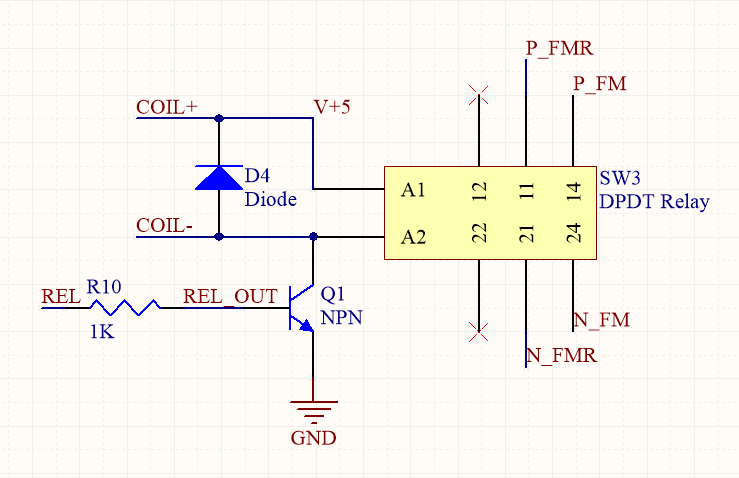
\includegraphics[width=150mm, keepaspectratio]{figures/wifisocket-relay.png}
	\caption{A rel�t kapcsol� �ramk�r}
	\label{fig:wifisocket-relay} 
\end{figure}

A h�l�zati �ram kapcsol�s�ra egy Schrack RTE24005 DPDT (k�t p�lus, k�t �ramk�r) rel� ker�lt felhaszn�l�sra (\ref{fig:wifisocket-relay}-es �bra). A k�t kapcsolt �ramk�r a null �s a f�zis, a k�t p�lus k�z�l az egyik a h�l�zatra kapcsol�dik, a m�sik a leveg�ben l�g. A rel� 250VAC-ra �s 8A-es terhel�sre van m�retezve. A bels� tekercs aktiv�l�s�hoz sz�ks�ges 5V-ot egy bipol�ris tranzisztorral kapcsolom, mivel a rel� �ramfelv�tele 80mA, viszont a mikrokontroller csak 12mA-ig terhelhet�.
A kikapcsol�skor a tekercsen maradt �ram elvezet�s�r�l flyback di�da gondoskodik.  

%----------------------------------------------------------------------------
\section{Szofver}
%----------------------------------------------------------------------------

\begin{figure}[!ht]
	\centering
	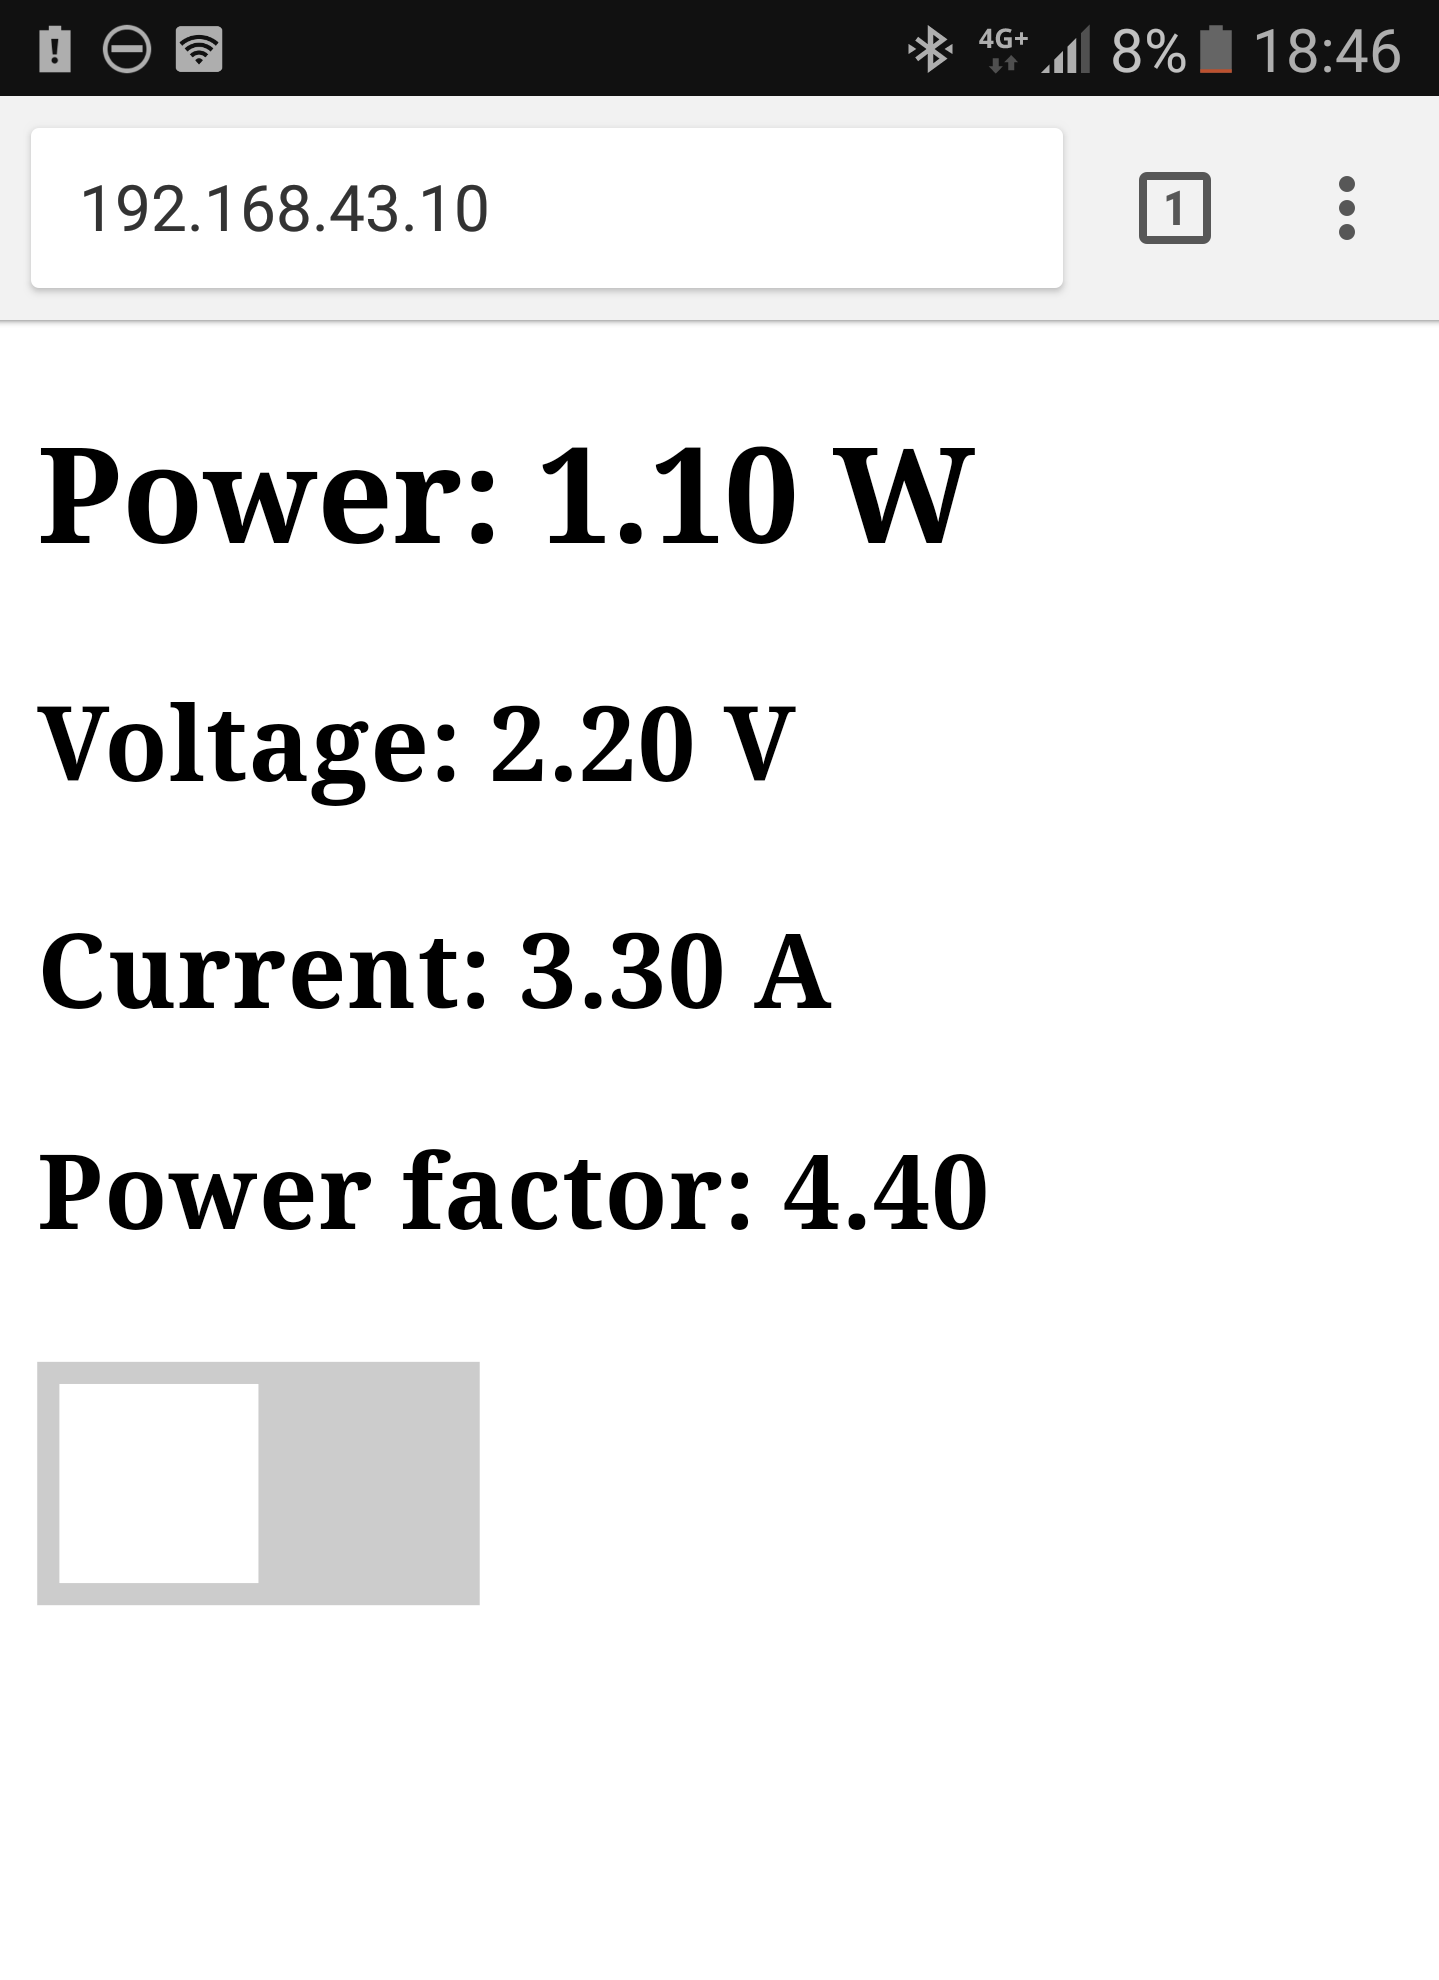
\includegraphics[width=150mm, height=150mm, keepaspectratio]{figures/wifisocket-webpage.png}
	\caption{A programozhat� aljzat f�oldala}
	\label{fig:wifisocket-webpage}
\end{figure}

%----------------------------------------------------------------------------
\section{Param�teres interface}
%----------------------------------------------------------------------------

\label{sec:parameters}

A h�l�zatba kapcsolt eszk�z�k programozhat�s�g�t nagy m�rt�kben megk�nny�ti, ha azok k�v�lr�l n�zve bizonyos szempontb�l egys�gesek. Az absztrakci� lehet egy, az eszk�zh�z hozz�rendelt param�terek halmaza, amelyek olvashat�ak �s esetenk�nt �rhat�ak is. P�ld�ul a pillanatnyi teljes�tm�nyt a power v�ltoz� tartalmazza, ami csup�n olvashat�. Az hogy egy param�ter k�v�lr�l v�ltoz�nak t\H{u}nik, nem jelenti felt�tlen�l azt, hogy az az eszk�z�n bel�l mind�g el�rhet�, lehet az egy lek�rdez�s �ltal megind�tott folyamat (legt�bb esetben m�r�s) eredm�nye is. Azon funkci�k amik beavatkoznak a k�rnyezetbe, �rhat� v�ltoz�kk�nt reprezent�lhat�ak.
A rel� �ll�sa a relay v�ltoz�ba �rt 0 vagy 1 �rt�kkel �ll�that�. Innent�l kezdve a teljes rendszer a szolg�ltatott param�terek, mint v�ltoz�k manipul�l�s�val programozhat�ak.
Ez a protokol, b�r meglehet�sen rugalmas, az �sszes perif�ri�t szolga (slave) szerepbe k�nyszer�ti, mivel minden tranzakci�t (�r�st/olvas�st) a k�zponti egys�g kezdem�nyez. Ha valamelyik perif�ri�n lenyomott gombhoz akarok akci�t rendelni, akkor ezt csak �gy tehetem meg ha a hozz�rendelt v�ltoz�t a m�sik eszk�zr�l pollolom, ami valamekkora id�vesztes�ggel j�r.

A kiolvas�s az WiFi-s eszk�z �ltal biztos�tott JSON (JavaScript Object Notation) interface-en kereszt�l t�rt�nik. A JSON egy ember �ltal is olvashat� sz�veges le�r�szabv�ny, ami az XML mellet a web legelterjedtebb form�tuma. Az �n implement�ci�mban csak az �sszes v�ltoz� egyidej\H{u} lek�rdez�s�re van lehet�s�g, de a visszafele kompatibilit�st megtartva hozz� lehetne adni a protokolhoz a v�ltoz�kra t�rt�n� sz\H{u}r�s lehet�s�g�t. A szenzor �ltal biztos�tott JSON oldal:

\begin{lstlisting}
{
	"relay": "0",
	"led": "1",
	"power": "0.00",
	"voltage": "0.00",
	"current": "0.00",
	"powerfactor": "0.00"
} 
\end{lstlisting}

A param�terek �r�s�hoz a HTTP (Hypertext Transfer Protocol) GET vagy POST met�dusa haszn�lhat� a /control oldalnak �tadva. A GET param�terek c�msorba k�dolhat�ak: 
\begin{lstlisting}
http://192.168.0.20/control?relay=1&led=0
\end{lstlisting}

A v�ltoztat�sok �rv�nyre jut�s�t az eszk�z a ,,Done'' �zenettel jelzi. Abban az esetban, ha b�rmi hiba mer�l fel az eszk�zzel kapcsolatban, nagyobb annak a val�sz�n\H{u}s�ge, hogy v�laszolni se tud az �zenetre.

\begin{table}[ht]
	\footnotesize
	\centering
	\caption{A Programozhat� aljzat param�terei}
	\begin{tabular}{|l|l|l|l|}
		\hline
		\textbf{N�v} & \textbf{Hozz�f�r�s} 	& \textbf{T�pus} & \textbf{Le�r�s}  \\ 
		\hline
		relay & �rhat�/olvashat� & boolean & a rel� �llapota \\
 		\hline
 		led & �rhat�/olvashat� & boolean & led �llapota \\
 		\hline
 		power & olvashat� & float & teljes�tm�ny (W) \\
 		\hline
 		voltage & olvashat� & float & fesz�lts�g (V) \\
 		\hline
 		current & olvashat� & float & �ram (A)\\
 		\hline
 		powerfactor & olvashat� & float & teljes�tm�ny t�nyez� \\
 		\hline		
	\end{tabular} 
\end{table}


%----------------------------------------------------------------------------
\section{HTML oldal}
%----------------------------------------------------------------------------

A k�zvetlen�l ember sz�m�ra is haszn�lhat� f�oldal kialak�t�s�nal az AJAX (Asynchronous JavaScript and XML) technik�t alkalmaztam. A m�dszertan l�nyege, hogy a weboldal �jrat�lt�se n�lk�l, az oldal tartalma v�ltozik dinamikusan. Az adatok fogad�sa �s k�ld�se asszinkron m�don, a szerver (mikrokontroller) fele t�rt�n� folyamatos kommunik�ci�val val�sul meg, kihaszn�lva a DOM (Document Object Model) ny�jtotta funkci�kat. (\ref{fig:wifisocket-webpage}-es �bra)

\lstinputlisting[language=HTML]{source/wifisocketMain.txt}

A onSwitch() f�ggv�ny felel�s a felhaszn�l� �ltal megnyomott kapcsol� �llapot�nak jelz�se az eszk�z fel�. Az refreshData() f�ggv�ny az eszk�z �llapot�nak v�ltoz�sa alapj�n friss�ti az weboldalt. Ez el�bbi a /control az ut�bbi a /json aloldal szolg�ltat�sait haszn�lja. 
%----------------------------------------------------------------------------
\section{Protot�pus}
%----------------------------------------------------------------------------

\begin{figure}[!ht]
	\centering
	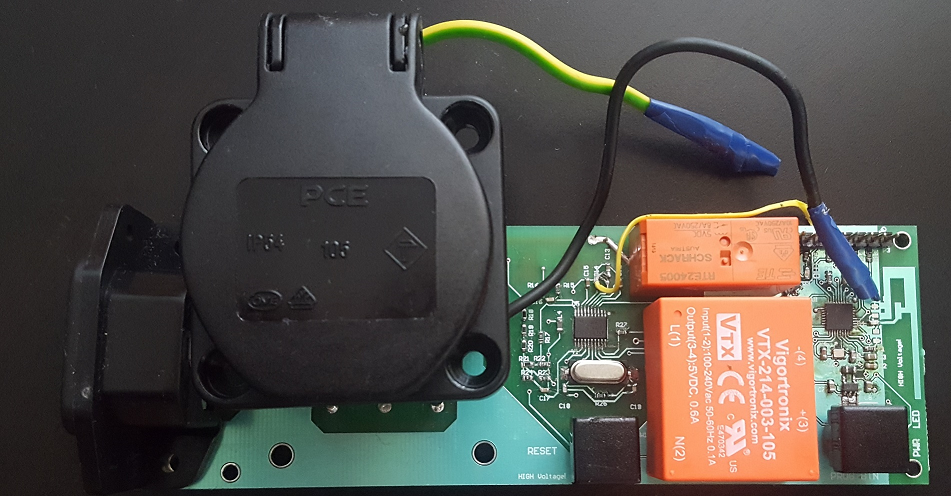
\includegraphics[width=150mm, keepaspectratio]{figures/wifisocket-proto.png}
	\caption{A programozht� aljzat protot�pusa} 
\end{figure}

Az eszk�z �leszt�se �s tesztel�se, mivel h�l�zati fesz�lts�gr�l m\H{u}k�dik, kiemelt figyelmet �s �vatoss�got ig�nyelt. A nagyfesz�lts�g\H{u} vezet�kekre nem ker�lt forraszt�sg�tl� maszk, �gy lehet�s�g volt azok �nnal t�rt�n� megvastag�t�s�ra. Ez garant�lta, hogy z�rlat eset�n az olvad�biztos�t�k aktiv�l�djon, �n ne az �ramk�r �gjen el. A tervez�sn�l c�l volt, hogy k�ls�, 5V-os t�pr�l is m\H{u}k�dtethet� legyen az aljzat, el�seg�tve a felprogramoz�st �s a tesztel�st. 

%----------------------------------------------------------------------------
\subsection{Felmer�lt probl�m�k}
%----------------------------------------------------------------------------

A protot�pusomon a LM3670MF-3.3 (Buck converter) enged�lyez� jel�t f�ldre h�ztam t�p helyett. A hiba k�nnyen jav�that� volt �j huzaloz�s szik�vel t�rt�n� kialak�t�s�val.

Mivel a ESP8285 �s STPM10BTR k�z�tt kommunik�ci�n�l nincs se lev�laszt�s se szintilleszt�s, ez�rt az eredeti tervekkel ellent�tben, a teljes�tm�nym�r� is 3.3V-r�l ker�lt meghajt�sra.

%----------------------------------------------------------------------------
\subsubsection{Zavarjelens�g}
%----------------------------------------------------------------------------

\begin{figure}[!ht]
	\centering
	\begin{minipage}{0.45\textwidth}
		\centering
		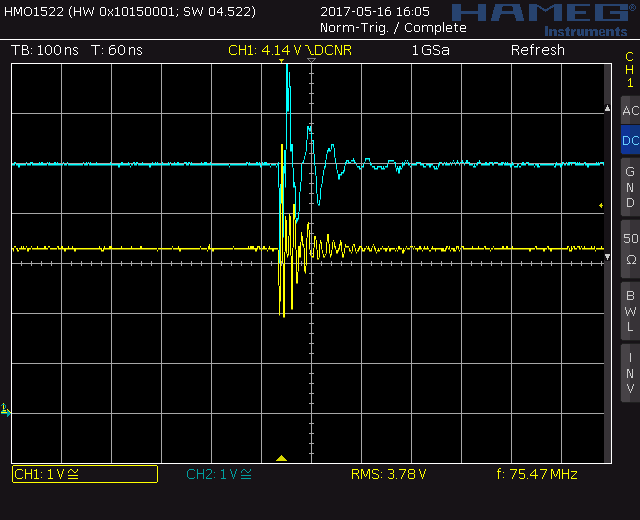
\includegraphics[width=0.9\textwidth]{figures/wifisocket-glitch1.png} % first figure itself
		\caption{first figure}
	\end{minipage}\hfill
	\begin{minipage}{0.45\textwidth}
		\centering
		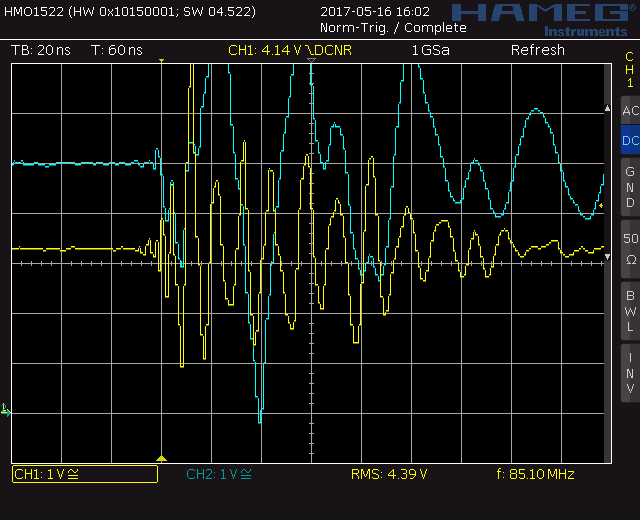
\includegraphics[width=0.9\textwidth]{figures/wifisocket-glitch2.png} % second figure itself
		\caption{second figure}
	\end{minipage}
\end{figure}

H�l�zatr�l t�rt�n� meghajt�s sor�n az eszk�z, a rel� z�r�sakor gyakran �jraindult. Hasonl� jelens�g csap�n a digitr�lis �g meghajt�sa sor�n nem l�pett fel, az �ramk�r megb�zhat�an m\H{u}k�d�tt. Az �jraindul�snak k�t oka lehet: 

\begin{itemize}  
	\item Zavarjel jut a reset l�bra, ami �jraind�tja a mikrokontrollert
	\item A t�p �tmenetileg az el��rt 3V al� esik
\end{itemize}

A hiba identifik�l�sa �rdek�ben k�t m�r�st v�geztem el:

\textbf{1. M�r�s:} Az eszk�zt lev�laszt� transzform�torra k�tve, oszcilloszk�pot k�t�ttem az 5V-os �s a 3.3V-os t�p�gra. A triggeresem�ny az 5V-os t�p jelent�s bezuhan�sa volt. L�that�, hogy a mindk�t t�pszinten jelent�s zavar (hozz�vet�legesen 150ns-ig fenn�ll� 50MHz-s csillap�tott oszcill�ci�) jelent meg. A 3.3V-os �g r�vid id�re beesett 2V al�. Ilyen frekvenci�n�l term�szetesen sz�m�t, hogy az �ramk�r mely pontj�n t�rt�nik a m�r�s, de felt�telezhet�, hogy ez a zavar mindenhol jelen van. R�ad�sul mindk�t fesz�lts�gszintet is t�bb konzdenz�tor sz\H{u}ri.
Az zavar m�g akkor sem cs�kkent �rdemben, amikor egy extra sz\H{u}r�kondenz�tort helyeztem az 5V-os �gra.



\textbf{2. M�r�s:} Kiz�rand� azt a lehet�s�get, hogy a Vigortronix t�pegys�g nem k�pes kezelni a rel� �ltal jelentett terhel�st, annak kapcsol��g�t egy, az �ramfelv�tel szempontj�b�l ekvivalens, ellen�ll�ssal helyettes�tettem. Ekkor a hiba megsz\H{u}nt, a t�pjelen csak minim�lis zaj volt �rz�kelhet�. 

A hib�t teh�t a nagyfesz�lts�g\H{u} r�sz, illetve a digit�lis logika interakci�ja okozza. Ezen zavarok megj�sl�sa szinte lehetetlen, gyakran k�ls� eredet\H{u}ek, ez�rt helyes tervez�ssel csup�n a kock�zatok cs�kkenthet�el, illetve a hat�sok m�rs�kelhet�ek:
\begin{itemize}  
	\item A digit�lis r�szek lehet� legt�volabb helyez�se a nagyfesz�lts�g\H{u} ter�letekt�l
	\item A digit�lis jelek galvanikus lev�laszt�sa
	\item Az integr�lt �ramk�r�k �s esetlegesen a huzaloz�s �rny�kol�sa
	\item Nagy potenci�lk�l�nbs�g\H{u} elemek a lehet� legt�volabb t�rt�n� elhelyez�se, vagy bev�g�s l�trehoz�sa az �ramk�r�n
\end{itemize}

Sajnos az �n esetemben az STPM10BTR nem f�ggetlen�thet� a t�pt�l, r�ad�sul a k�tir�ny� SPI-szer\H{u} kommunik�ci� miatt az ESP8285 se. Ez a probl�ma csak a ny�k �jratervez�s�vel lehetne jav�that�, emiatt teljes�tm�nym�r� konfigur�l�sa (kalibr�l�sa) elmaradt, illetve a rel� csak kisebb fesz�lts�get tud biztons�gosan kapcsolni.



%----------------------------------------------------------------------------
\chapter*{K�sz�netnyilv�n�t�s}\addcontentsline{toc}{chapter}{K�sz�netnyilv�n�t�s}
%----------------------------------------------------------------------------

Ez nem k�telez�, ak�r t�r�lhet� is. Ha a szerz� sz�ks�g�t �rzi, itt lehet k�sz�netet nyilv�n�tani azoknak, akik hozz�j�rultak munk�jukkal ahhoz, hogy a hallgat� a szakdolgozatban vagy diplomamunk�ban le�rt feladatokat sikeresen elv�gezze. A konzulensnek val� k�sz�netnyilv�n�t�s sem k�telez�, a konzulensnek hivatalosan is dolga, hogy a hallgat�t konzult�lja.



\addcontentsline{toc}{chapter}{Irodalomjegyz�k}
\bibliographystyle{unsrt}
\bibliography{mybib}

%----------------------------------------------------------------------------
\appendix
%----------------------------------------------------------------------------
\chapter*{F�ggel�k}\addcontentsline{toc}{chapter}{F�ggel�k}
\setcounter{chapter}{6}  % a fofejezet-szamlalo az angol ABC 6. betuje (F) lesz
\setcounter{equation}{0} % a fofejezet-szamlalo az angol ABC 6. betuje (F) lesz
\numberwithin{equation}{section}
\numberwithin{figure}{section}
\numberwithin{lstlisting}{section}
%\numberwithin{tabular}{section}

\begin{figure}[!ht]
	\centering
	
\includegraphics[width=150mm, keepaspectratio]{figures/placeholder.png}
	\caption{Az elk�sz�lt rendeszer (kell egy fot�)} 
\end{figure}

\begin{figure}[!ht]
	\centering
	
\includegraphics[width=150mm, keepaspectratio]{figures/placeholder.png}
	\caption{A k�zponti egys�g f�oldala (kell egy screenshot)} 
\end{figure}

\begin{figure}[!ht]
	\centering
	
\includegraphics[width=150mm, keepaspectratio]{figures/placeholder.png}
	\caption{A k�zponti egys�g be�ll�t�sai (kell egy screenshot)} 
\end{figure}

\begin{figure}[!ht]
	\centering
	
\includegraphics[width=150mm, keepaspectratio]{figures/placeholder.png}
	\caption{A k�zponti egys�g programoz� oldala (kell egy screenshot)} 
\end{figure}

\begin{figure}[!ht]
\centering
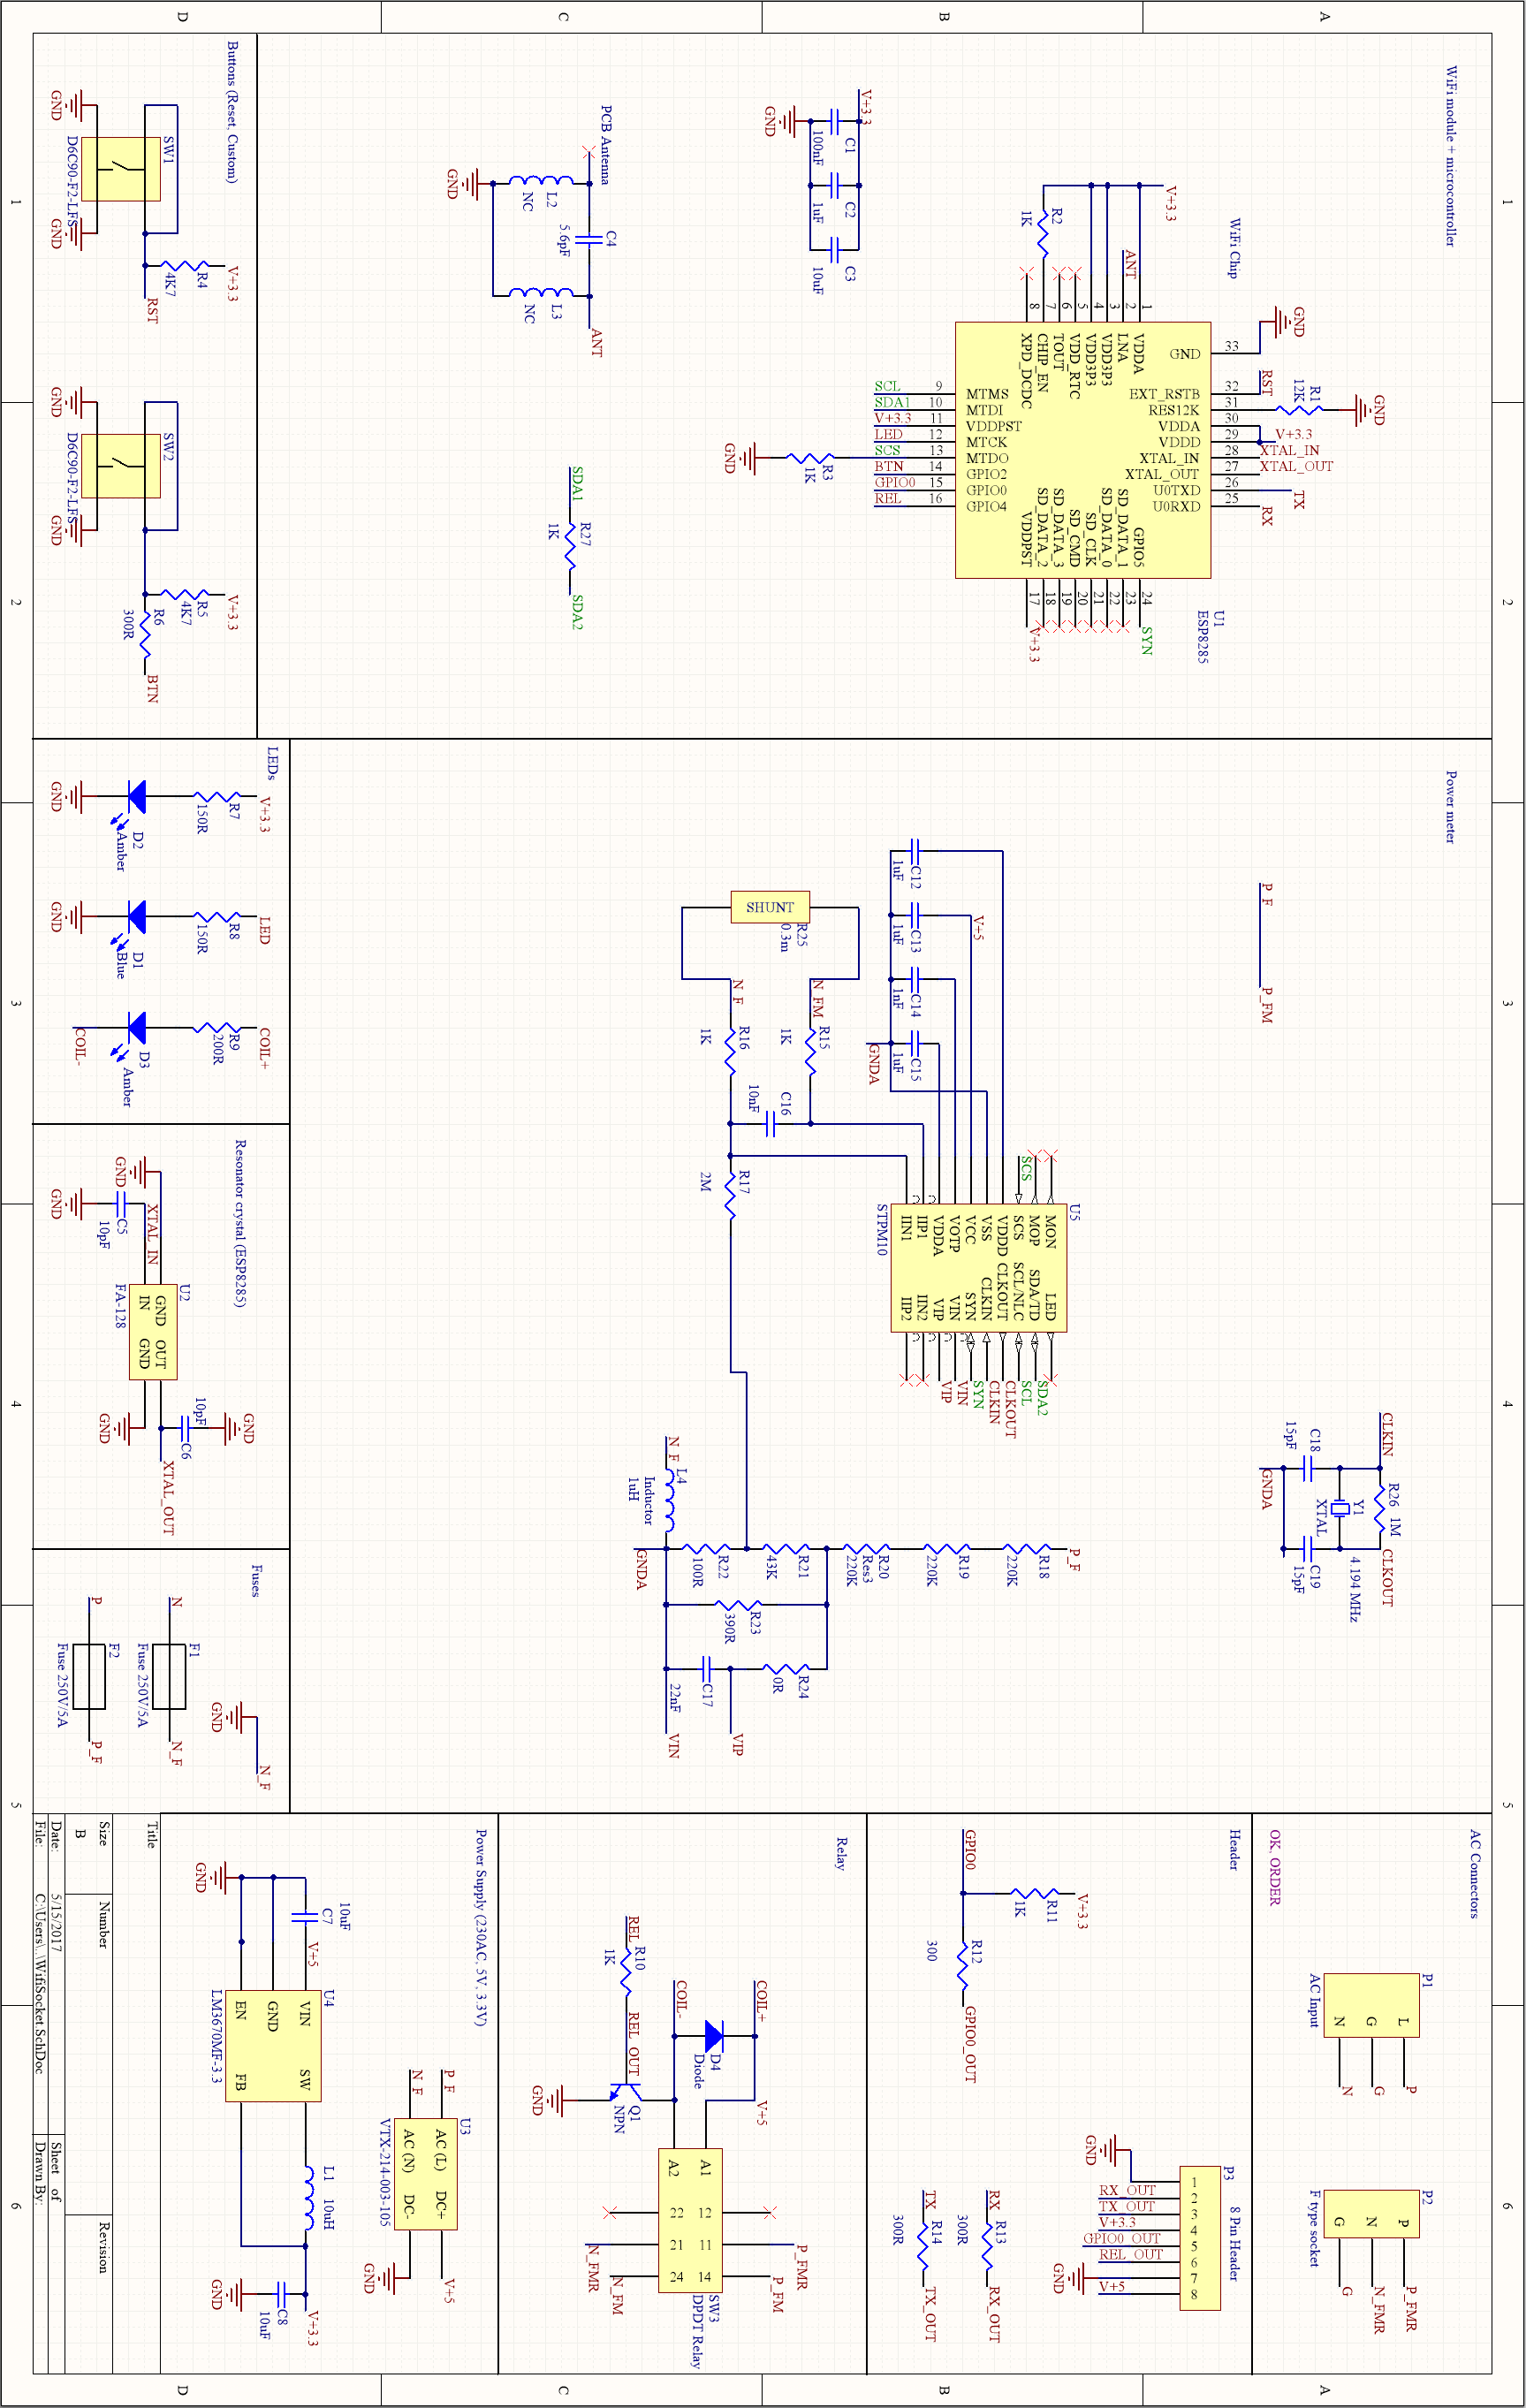
\includegraphics[width=150mm, keepaspectratio]{figures/wifisocket-sch-full.png}
\caption{A programozhat� aljzat kapcsol�si rajza} 
\end{figure}

\begin{figure}[!ht]
	\centering
	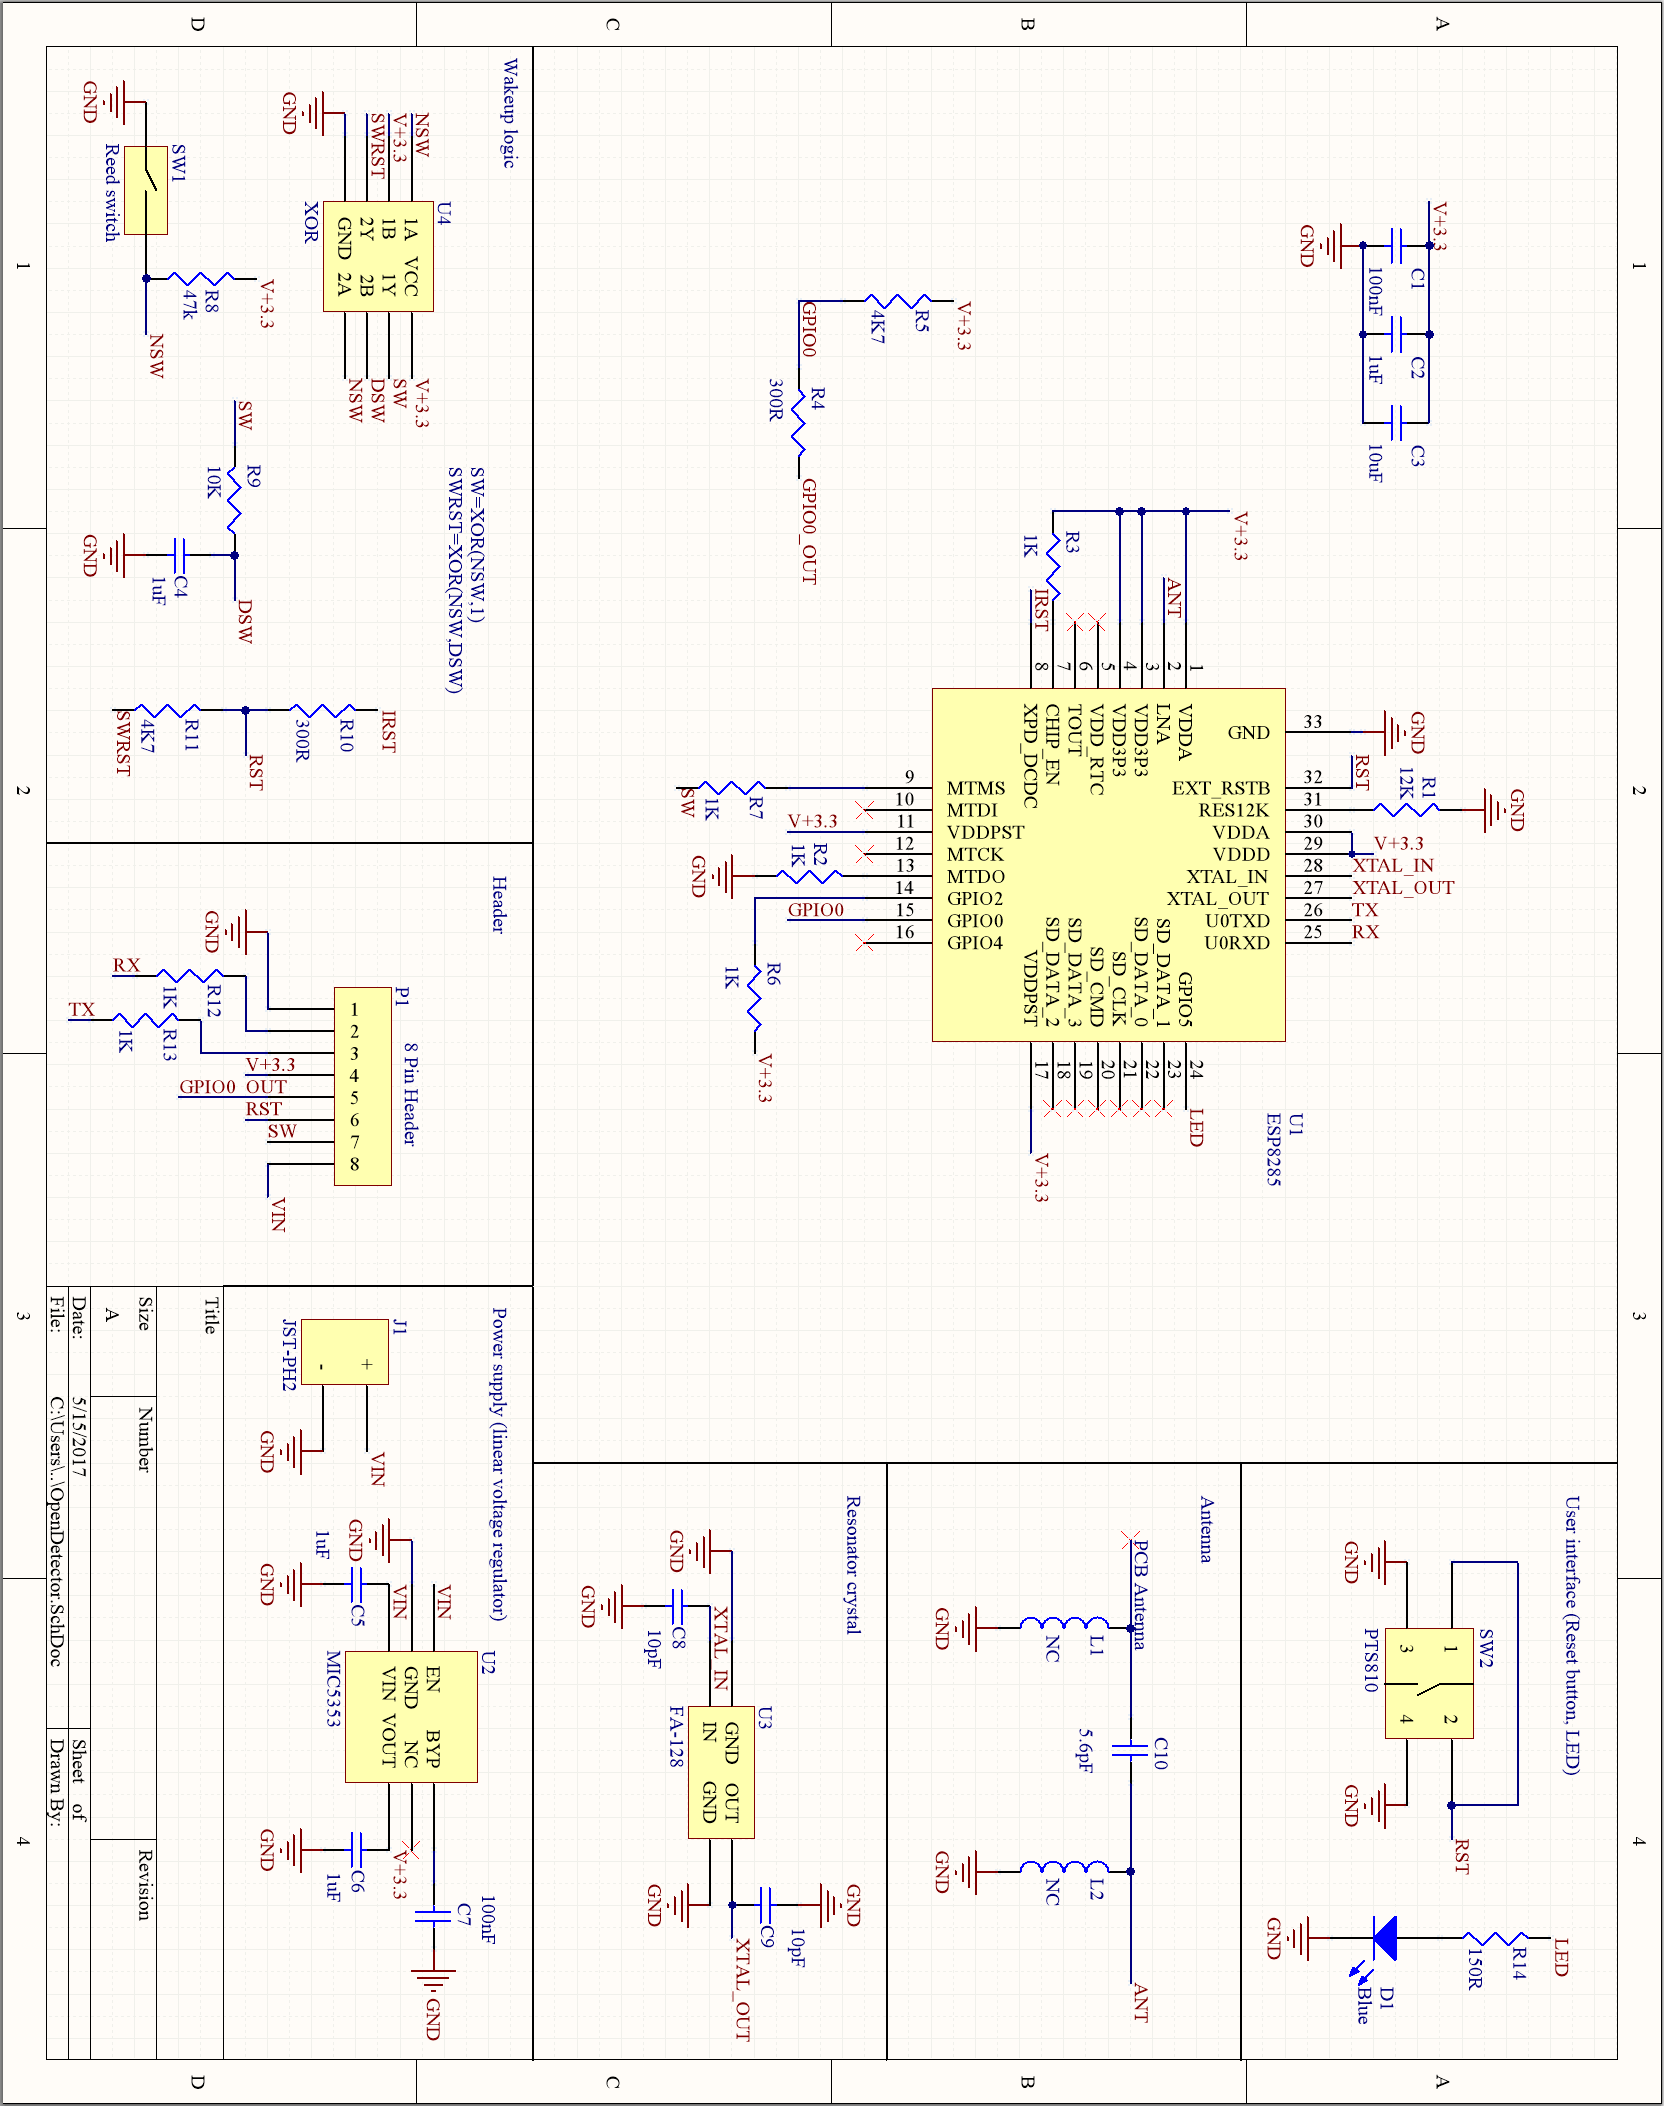
\includegraphics[width=150mm, keepaspectratio]{figures/opendetector-sch-full.png}
	\caption{A nyit�s�rz�kel� kapcsol�si rajza} 
\end{figure}

\begin{figure}[!ht]
	\centering
	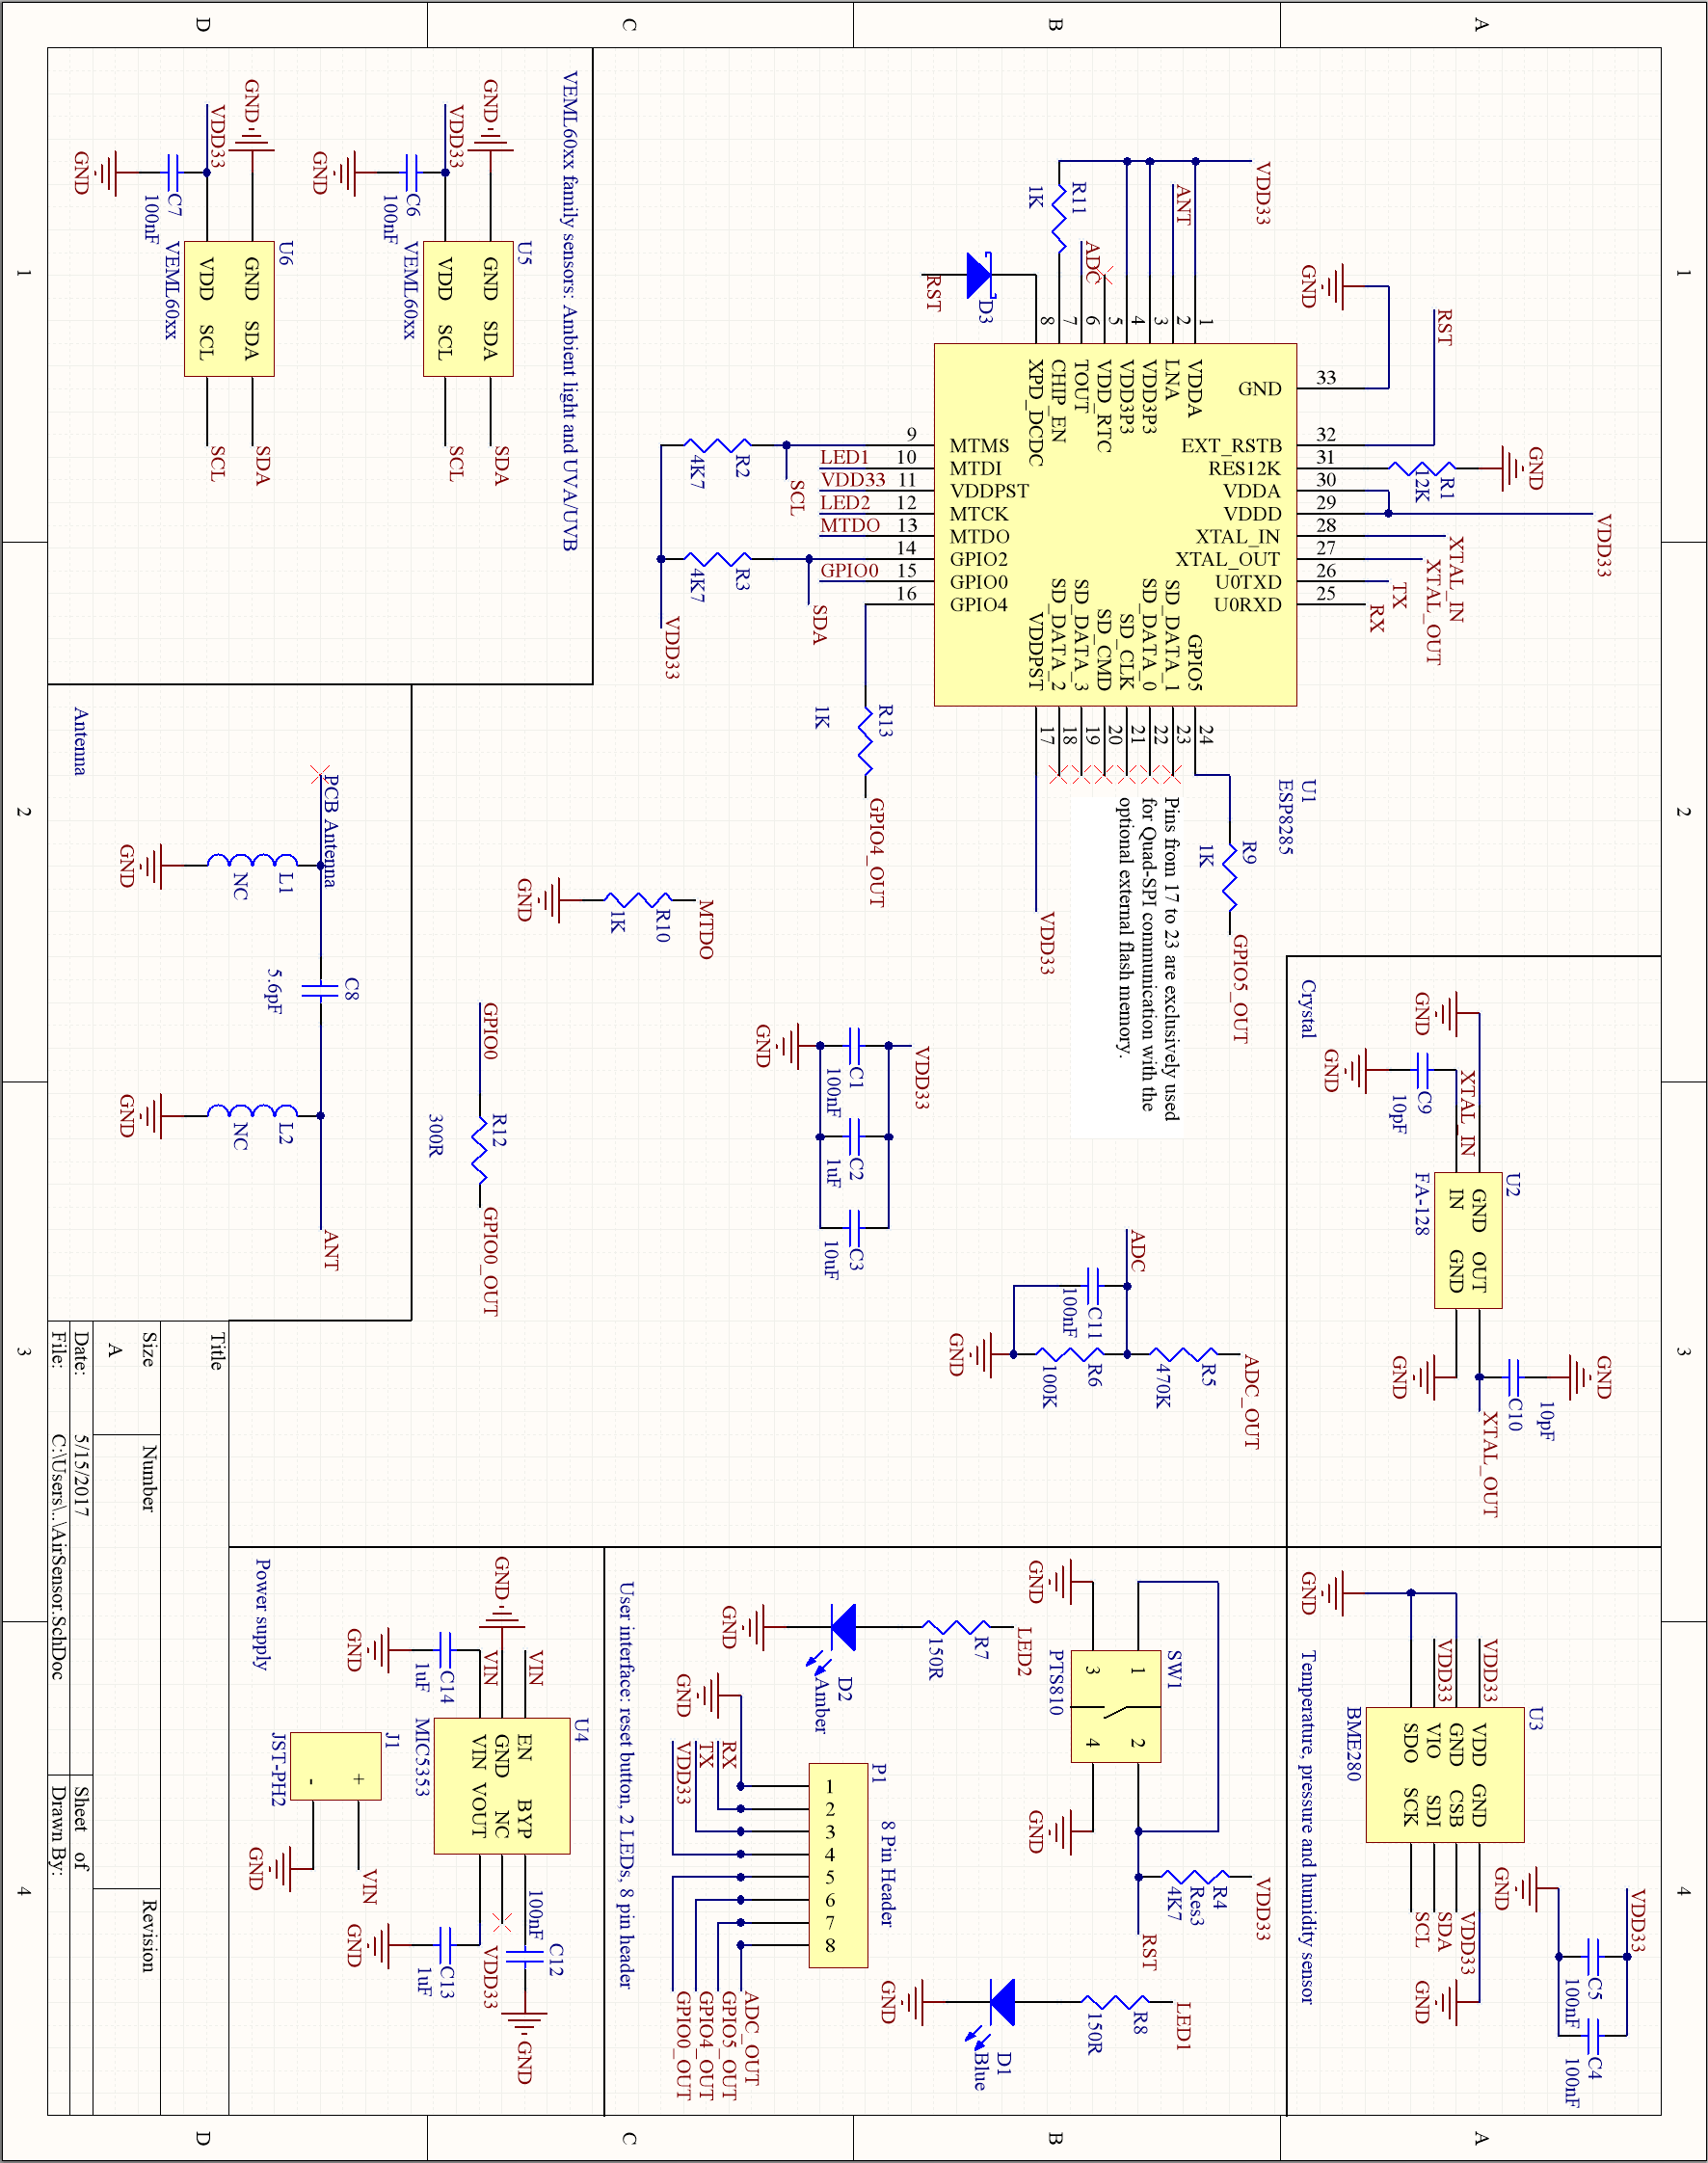
\includegraphics[width=150mm, keepaspectratio]{figures/enviromental-sensor-sch-full.png}
	\caption{A k�rnyezeti szenzor kapcsol�si rajza} 
\end{figure}








\label{page:last}
\end{document}
